\documentclass[12pt,a4paper,twoside]{book}

% Essential packages
\usepackage{graphicx}
\usepackage{setspace}
\usepackage[numbers,sort&compress]{natbib}
\usepackage[english]{babel}
\usepackage[utf8]{inputenc}
\usepackage{color}
\usepackage{hhline}
\usepackage{multirow}
\usepackage{acronym}
\usepackage{hyperref}
\usepackage{amsmath,amssymb}
\usepackage{fancyhdr}
\usepackage{epsfig}
\usepackage{algorithm}
\usepackage{algorithmic}
\usepackage{longtable}
\usepackage{caption}
\usepackage{tikz}
\usepackage{adjustbox}
\usepackage{listings}
\usepackage{xcolor}
\usepackage{booktabs}
\usepackage{float}
\usepackage{subcaption}
\usetikzlibrary{arrows.meta, positioning, shapes.geometric, calc, fit, backgrounds}

% Code listing configuration
\lstset{
    basicstyle=\ttfamily\small,
    breaklines=true,
    frame=single,
    backgroundcolor=\color{gray!10},
    keywordstyle=\color{blue},
    commentstyle=\color{green!50!black},
    stringstyle=\color{red!60!black},
    numbers=left,
    numberstyle=\tiny\color{gray},
    numbersep=5pt,
    showstringspaces=false,
    tabsize=2
}

\lstdefinelanguage{Python}{
    keywords={def, class, return, if, else, elif, for, while, with, as, import, from, async, await, try, except, finally, raise, True, False, None, and, or, not, in, is, lambda, yield},
    keywordstyle=\color{blue}\bfseries,
    ndkeywords={self, cls, BaseModel, Field, Literal, Optional, Union, list, dict, str, int, float, bool},
    ndkeywordstyle=\color{purple},
    sensitive=true,
    comment=[l]{\#},
    morestring=[b]",
    morestring=[b]',
}

% Hyperref configuration
\hypersetup{
    linktocpage=true,
    colorlinks=true,
    linkcolor=blue,
    citecolor=blue,
    urlcolor=blue,
    pdftitle={Multi-Agent System for Automated Fact-Checking of YouTube Videos},
    pdfauthor={Begona Echavarren Sanchez}
}
\definecolor{Hgray}{gray}{0.6}

% Page layout
\setlength{\topmargin}{0cm}
\setlength{\textheight}{23cm}
\setlength{\textwidth}{17cm}
\setlength{\oddsidemargin}{0cm}
\setlength{\evensidemargin}{0cm}
\setlength{\headheight}{1cm}

% Section numbering depth
\setcounter{secnumdepth}{3}
\setcounter{tocdepth}{1}

\makeatletter
\renewcommand{\l@section}[2]{%
  \addpenalty{-\@highpenalty}%
  \vskip 1.0em \@plus\p@%
  \@dottedtocline{0}{0em}{1.5em}{#1}{#2}%
}
\renewcommand{\l@subsection}{\@dottedtocline{1}{1.5em}{2.3em}}
\renewcommand{\l@subsubsection}{\@dottedtocline{2}{3.8em}{3.2em}}
\makeatother

\raggedbottom

% Algorithm settings
\renewcommand{\algorithmicrequire}{\textbf{Input:}}
\renewcommand{\algorithmicensure}{\textbf{Output:}}

%%%%%%%%%%%%
% DOCUMENT %
%%%%%%%%%%%%
\begin{document}

\setcounter{section}{0}
\renewcommand{\thesection}{\arabic{section}}

% Title page
\newpage
\thispagestyle{empty}

\baselineskip 2em

\centerline{\includegraphics[width=0.6\textwidth]{images/UOC-logo}}
\begin{center}
\textsc{Universitat Oberta de Catalunya (UOC) \\
Master's Degree in Data Science \\
}

\vspace*{1.5cm}

\textsc{\Large MASTER'S THESIS}

\vspace*{0.5cm}

\textsc{\large Area: Natural Language Processing}

\vspace*{2.0cm}

\textbf{\Large Factible: A Multi-Agent System for Automated Fact-Checking of YouTube Videos}

\vspace{2.5cm}
\baselineskip 1em

\baselineskip 2em
-----------------------------------------------------------------------------\\
Author: Bego\~na Echavarren S\'anchez\\
Tutor: Josep-Anton Mir Tutusaus\\
-----------------------------------------------------------------------------\\
\vspace*{1.5cm}
December 2025

\end{center}

\newpage
\pagestyle{empty}
\hfill

\newpage

% Front matter
\pagenumbering{roman}
\setcounter{page}{1}
\pagestyle{plain}

%%%%%%%%%%%%%%%%
%%% COPYRIGHT %%%
%%%%%%%%%%%%%%%%
\chapter*{Copyright}

This work is licensed under a Creative Commons Attribution-NonCommercial-NoDerivatives 4.0 International License.

\vspace{1cm}

\begin{figure}[ht]
\centering
\includegraphics[scale=1]{images/license.png}
\end{figure}

Attribution-NonCommercial-NoDerivatives 4.0 International (CC BY-NC-ND 4.0)

\href{https://creativecommons.org/licenses/by-nc-nd/4.0/}{https://creativecommons.org/licenses/by-nc-nd/4.0/}

\vspace{1cm}

\textbf{Source Code:}

The complete source code for this project is publicly available at:

\url{https://github.com/begoechavarren/factible}

%%%%%%%%%%%%%
%%% RECORD %%%
%%%%%%%%%%%%%
\chapter*{FINAL PROJECT RECORD}

\begin{table}[ht]
\centering{}
\renewcommand{\arraystretch}{2}
\begin{tabular}{r | l}
\hline
Title of the project: & Factible: A Multi-Agent System for Automated\\
 & Fact-Checking of YouTube Videos\\
\hline
Author's name: & Bego\~na Echavarren S\'anchez\\
\hline
Tutor's name: & Josep-Anton Mir Tutusaus\\
\hline
Delivery date: & 12/2025\\
\hline
Degree or program: & Master's Degree in Data Science\\
\hline
Final Project area: & Natural Language Processing\\
\hline
Language of the project: & English\\
\hline
Keywords: & fact-checking, LLM, multi-agent systems\\
\hline
\end{tabular}
\end{table}

%%%%%%%%%%%%%%%%%%%
%%% ACKNOWLEDGEMENTS %%%
%%%%%%%%%%%%%%%%%%%
\chapter*{Acknowledgements}

I would like to express my sincere gratitude to my tutor, Josep-Anton Mir Tutusaus, for his guidance, insightful feedback, and continuous support throughout this project. His expertise in data science and machine learning was invaluable in shaping this work.

I am also grateful to the Universitat Oberta de Catalunya (UOC) for providing an excellent learning environment and the resources necessary to complete this Master's Degree in Data Science.

Special thanks to the open-source community, particularly the developers of Pydantic AI, FastAPI, and the various tools that made this implementation possible. The availability of high-quality open-source software was essential to this project's success.

Finally, I would like to thank my family and friends for their patience, encouragement, and understanding during the intensive months of this thesis work.

%%%%%%%%%%%%%%%%
%%% ABSTRACT %%%
%%%%%%%%%%%%%%%%
\chapter*{Abstract}
\addcontentsline{toc}{chapter}{Abstract}

\onehalfspacing

Misinformation on video platforms represents a growing challenge in the digital age. YouTube, with over 2 billion monthly users and 500 hours of video uploaded every minute, serves as a primary information source for millions worldwide. However, the absence of effective verification mechanisms allows false or misleading claims to spread at massive scale, impacting public health, democratic processes, and social cohesion.

This thesis presents Factible, a multi-agent system for automated fact-checking of YouTube videos. The system implements an end-to-end pipeline that processes video content through five specialized components: transcript extraction, claim detection using thesis-first reasoning, query generation for evidence retrieval, open-web evidence collection with source reliability assessment, and verdict synthesis with confidence levels.

The implementation leverages large language models (LLMs) for reasoning tasks while employing classical algorithms for deterministic operations. Key innovations include a thesis-first approach for claim importance ranking, adaptive credibility filtering for source quality, and a three-level parallelization architecture for latency optimization.

Evaluation on 30 annotated YouTube videos across health, climate, and political topics demonstrates strong performance: 81.3\% claim extraction precision, 94.7\% evidence retrieval success rate, and 73.3\% verdict accuracy. The system achieves practical efficiency with mean processing time of 129.6 seconds per video at \$0.003 average cost, enabling cost-effective deployment for individual users.

The complete system, including a web-based interface with real-time streaming, is publicly available as open-source software, bridging the gap between academic research and practical fact-checking tools accessible to non-expert users.

\vspace{0.5cm}

\textbf{Keywords}: automated fact-checking, large language models, multi-agent systems, natural language processing, misinformation detection, YouTube, information retrieval, evidence-based verification

\newpage

% Header/footer configuration
\pagestyle{fancy}
\renewcommand{\chaptermark}[1]{\markboth{#1}{}}
\renewcommand{\sectionmark}[1]{\markright{\thesection.\ #1}}
\lhead[\fancyplain{}{\bfseries\thepage}]{\fancyplain{}{\bfseries\rightmark}}
\rhead[\fancyplain{}{\bfseries\leftmark}]{\fancyplain{}{\bfseries\thepage}}
\cfoot{}

% Table of contents
\cleardoublepage
\phantomsection
\addcontentsline{toc}{chapter}{Table of Contents}
\tableofcontents

% List of figures
\cleardoublepage
\phantomsection
\addcontentsline{toc}{chapter}{List of Figures}
\listoffigures

% List of tables
\cleardoublepage
\phantomsection
\addcontentsline{toc}{chapter}{List of Tables}
\listoftables

\thispagestyle{empty}

% Reset header/footer
\pagestyle{fancy}
\renewcommand{\chaptermark}[1]{\markboth{#1}{}}
\renewcommand{\sectionmark}[1]{\markright{\thesection.\ #1}}
\lhead[\fancyplain{}{\bfseries\thepage}]{\fancyplain{}{\bfseries\rightmark}}
\rhead[\fancyplain{}{\bfseries\leftmark}]{\fancyplain{}{\bfseries\thepage}}
\cfoot{}

\onehalfspacing

%%%%%%%%%%%%%%%%%%%%%%%%%%%%%%%%%%%%%%%%%%%%%%%%%%%%%%%
% MAIN CONTENT
%%%%%%%%%%%%%%%%%%%%%%%%%%%%%%%%%%%%%%%%%%%%%%%%%%%%%%%

\mainmatter
\cleardoublepage
\markboth{}{}

% Chapter 1: Introduction
%%%%%%%%%%%%%%%%%%%%%%%%%%%%%%%%%%%%%%%%%%%%%%%%%%%%%%%
% CHAPTER 1: INTRODUCTION
%%%%%%%%%%%%%%%%%%%%%%%%%%%%%%%%%%%%%%%%%%%%%%%%%%%%%%%
\section{Introduction}

Misinformation on digital platforms has become a major challenge in the information age. YouTube, with over 2 billion monthly active users, has evolved into a primary information source for millions of people worldwide. However, the absence of effective verification mechanisms allows false or misleading claims to propagate at massive scale, impacting public health, democratic processes, and social cohesion \citep{wardle2017information, benkler2018network}.

This thesis addresses the critical need for automated fact-checking systems capable of processing video content from platforms like YouTube. The project develops Factible, a multi-agent system that implements an end-to-end pipeline for extracting, verifying, and synthesizing factual claims from YouTube videos using large language models (LLMs) and web-based evidence retrieval.

%-------------------------------------------------------
\subsection{Context and Motivation}
%-------------------------------------------------------

\subsubsection{The Problem of Video Misinformation}

The central problem this project addresses is the \textbf{lack of automated, accessible mechanisms to verify factual claims in audiovisual content from digital platforms}, specifically YouTube videos. Individual users lack tools to systematically verify claims, while manual verification requires advanced skills, considerable time, and resources that are not always available.

YouTube presents unique challenges for fact-checking:

\begin{itemize}
    \item \textbf{Scale}: Over 500 hours of video are uploaded every minute, making human-only verification impossible.
    \item \textbf{Consumption patterns}: Videos are consumed passively, with viewers less likely to critically evaluate claims than when reading text.
    \item \textbf{Lack of annotation}: Unlike text articles, videos do not come with metadata identifying factual claims.
    \item \textbf{Temporal context}: Claims are embedded in a narrative flow, making extraction and verification more complex than isolated text statements.
\end{itemize}

\subsubsection{Relevance and Importance}

This project is relevant for multiple reasons:

\begin{itemize}
    \item \textbf{Social impact}: Misinformation erodes trust in institutions, influences political decisions, and affects public health \citep{wardle2017information, benkler2018network}. An automated verification system can contribute to mitigating these effects by enabling faster, more accessible fact-checking.

    \item \textbf{Technological challenge}: The project integrates multiple areas of data science research: natural language processing, information retrieval, source credibility evaluation, and automated reasoning. It represents a technically complex problem requiring innovative solutions.

    \item \textbf{Scalability necessity}: The volume of content generated daily makes purely human fact-checking infeasible. Automation is necessary to address the problem at scale, serving as a force multiplier for human fact-checkers.

    \item \textbf{Media literacy}: Tools that empower citizens to critically evaluate information promote critical thinking and strengthen media literacy in society, contributing to a healthier information ecosystem.
\end{itemize}

\subsubsection{Current State of Solutions}

Currently, three main approaches exist for fact-checking:

\begin{enumerate}
    \item \textbf{Manual fact-checking}: Organizations like Newtral, Maldita.es, PolitiFact, and FactCheck.org employ specialized journalists. This approach guarantees quality but is limited by human resources and is inherently slow, typically checking only a few claims per day.

    \item \textbf{Academic systems}: Projects like FEVER \citep{thorne2018fever}, FEVEROUS \citep{aly2021feverous}, and recent work on scientific verification \citep{wadden2020scifact} operate primarily on structured knowledge bases (Wikipedia) or require specifically curated datasets. They are not available as products usable by end users and have limited scope.

    \item \textbf{Verification APIs}: Google Fact Check Tools API aggregates fact-checks already published by professional organizations but only covers content previously verified manually. It does not provide new verification for unexamined content.
\end{enumerate}

\textbf{Identified gap}: None of these approaches provides automated end-to-end verification for continuously generated audiovisual content on platforms like YouTube. A gap exists between academic research (static datasets, limited domains) and practical, accessible tools for end users.

%-------------------------------------------------------
\subsection{Project Objectives}
%-------------------------------------------------------

\subsubsection{Main Objective}

Design, implement, and evaluate a multi-agent system based on language models capable of automatically verifying factual claims in YouTube videos through retrieval and analysis of web-based evidence, generating substantiated verdicts with confidence estimates that are useful for end users.

\subsubsection{Specific Objectives}

\begin{enumerate}
    \item \textbf{Multi-agent architecture design}
    \begin{itemize}
        \item Define a modular processing pipeline with specialized components
        \item Establish structured data schemas for communication between agents
        \item Design the information orchestration system
    \end{itemize}

    \item \textbf{System component implementation}
    \begin{itemize}
        \item Develop the module for extracting video transcripts from YouTube
        \item Implement the claim identification agent with relevance classification
        \item Create the optimized search query generator
        \item Develop the web scraping system with source reliability evaluation
        \item Implement the generator for explainable and traceable verdicts
    \end{itemize}

    \item \textbf{LLM usage optimization}
    \begin{itemize}
        \item Compare performance between commercial models (e.g., GPT-4o-mini) and open-source alternatives (e.g., Qwen 3, DeepSeek)
        \item Analyze trade-offs between cost, latency, and output quality
        \item Evaluate prompt optimization strategies and structured outputs
    \end{itemize}

    \item \textbf{System evaluation}
    \begin{itemize}
        \item Define technical performance metrics: response time, cost per token, throughput, and completion rate per agent
        \item Include LLM-specific quantitative metrics such as faithfulness, factual consistency, coherence, and stance accuracy
        \item Incorporate quantitative and qualitative evaluation with LLM-as-a-judge and manual review
        \item Conduct case studies across different video topics and analyze system limitations
    \end{itemize}

    \item \textbf{End-to-end system implementation}
    \begin{itemize}
        \item Develop a REST API with real-time streaming
        \item Create an intuitive web interface for end users
        \item Ensure reproducibility and generate documentation
    \end{itemize}

    \item \textbf{Ethical and bias considerations}
    \begin{itemize}
        \item Analyze potential biases in sources and models used
        \item Identify limitations of the automated approach, its possible impact on misinformation propagation, and define best practices to mitigate these risks during verification
    \end{itemize}
\end{enumerate}

\subsubsection{Project Scope}

\textbf{Includes:}
\begin{itemize}
    \item YouTube videos with available transcripts (automatic or manual subtitles)
    \item Factual claims verifiable through public web sources
    \item Content in English
    \item On-demand processing of individual videos
\end{itemize}

\textbf{Does not include:}
\begin{itemize}
    \item Self-generation of transcripts from audio (speech-to-text)
    \item Verification of visual content
    \item Large-scale batch verification
    \item Content from platforms other than YouTube
\end{itemize}

%-------------------------------------------------------
\subsection{Ethical Considerations and Social Impact}
%-------------------------------------------------------

\subsubsection{Ethical Commitment and Global Competence}

The project addresses three dimensions of ethical and global competence:

\textbf{(I) Sustainability}: The use of LLMs implies significant energy consumption. This is addressed through evaluation of local open-source models versus commercial cloud services, prompt optimization to minimize processed tokens, and transparent documentation of resource consumption.

\textbf{(II) Ethical behavior and social responsibility}: LLMs can perpetuate biases present in their training data. Mitigation strategies include:
\begin{itemize}
    \item Total transparency in consulted sources with verifiable URLs
    \item Presentation of evidence showing different stances (supports/refutes/neutral)
    \item Explicit evaluation of confidence level in each verdict
    \item Clear warnings about limitations of the automated system
\end{itemize}
The system positions itself as a support tool that automates preliminary steps, allowing professionals to focus on complex analyses requiring human judgment.

\textbf{(III) Diversity and human rights}: The system seeks to evaluate diversity of perspectives when multiple web sources with different approaches are available, documenting this limitation when not possible. It does not censor content but provides additional context through verification, respecting freedom of expression. It does not process personal data or identifiable user information.

\subsubsection{Sustainable Development Goals (SDGs)}

The project contributes to three SDGs from the 2030 Agenda:

\textbf{SDG 4 (Quality Education)}: The system acts as a media literacy tool that promotes critical thinking and the ability to evaluate information sources. It facilitates learning about fact-checking, evidence analysis, and recognition of verifiable claims---fundamental competencies in today's digital society.

\textbf{SDG 16 (Peace, Justice and Strong Institutions)}: It combats misinformation that erodes trust in democratic institutions and media. It provides transparent, traceable, and accessible verification mechanisms that allow citizens to systematically contrast factual claims, contributing to a healthier, more resilient information ecosystem.

\textbf{SDG 10 (Reduced Inequalities)}: It democratizes access to fact-checking through a free, open-source tool, reducing the gap between professional organizations with specialized resources (fact-checkers, journalists) and individual citizens. It empowers users without specialized training to critically evaluate content on digital platforms.

%-------------------------------------------------------
\subsection{Methodology}
%-------------------------------------------------------

\subsubsection{Research Strategy}

This project adopts a \textbf{Design and Creation} strategy \citep{oates2006}, appropriate for information systems research where a new technological artifact is developed whose construction and evaluation constitute the main contribution to knowledge. According to \citet{hevner2004}, this strategy requires: (1) creating a viable artifact, (2) addressing a relevant problem, (3) conducting rigorous evaluation, (4) making clear contributions, (5) applying rigor in construction, (6) designing as a search process, and (7) effectively communicating results.

\textbf{Data collection techniques for evaluation:}

\textit{Quantitative:}
\begin{itemize}
    \item Automated measurement of system metrics: processing time, cost (tokens $\times$ price), number of retrieved sources, stance distribution
    \item Evaluation using LLM-as-a-judge to assess quality of extracted claims and generated verdicts
    \item Multi-agent coordination metrics: task completion rate, latency per agent
\end{itemize}

\textit{Qualitative:}
\begin{itemize}
    \item Manual review of system outputs (claim relevance, verdict coherence)
    \item Detailed case studies across different topics
\end{itemize}

\subsubsection{Development Methodology}

\textbf{Chosen strategy}: Development of a new end-to-end product with a functional web interface.

\textbf{Justification}: This strategy is most appropriate because it allows evaluation of the complete practical viability of the system under real usage conditions, not just as a theoretical concept. Modular development from scratch facilitates experimentation with different LLM configurations and guarantees total control over the verification pipeline. Including a web interface demonstrates applicability for end users and allows collecting feedback on real system usability.

\textbf{Iterative development process:}
\begin{enumerate}
    \item Implementation of individual components with isolated testing
    \item End-to-end pipeline integration (functional MVP)
    \item Iterative refinement module by module based on results
    \item Comparative evaluation with different LLM configurations
\end{enumerate}

%-------------------------------------------------------
\subsection{Summary of Project Outputs}
%-------------------------------------------------------

This thesis produces the following outputs:

\begin{enumerate}
    \item \textbf{Factible}: A complete, open-source multi-agent fact-checking system for YouTube videos, available at \url{https://github.com/begoechavarren/factible}

    \item \textbf{Modular pipeline architecture}: Five specialized components (Transcriptor, Claim Extractor, Query Generator, Online Search, Output Generator) with well-defined interfaces

    \item \textbf{Web interface}: React-based frontend with real-time SSE streaming for interactive verification

    \item \textbf{REST API}: FastAPI-based backend enabling programmatic access to fact-checking functionality

    \item \textbf{Evaluation framework}: Infrastructure for systematic experimentation including tracking, metrics computation, and result analysis

    \item \textbf{Annotated evaluation dataset}: 30 YouTube videos with 503 ground truth claims across health, climate, and political topics

    \item \textbf{This thesis document}: Comprehensive documentation of the design, implementation, and evaluation of the system
\end{enumerate}


% Chapter 2: State of the Art
%%%%%%%%%%%%%%%%%%%%%%%%%%%%%%%%%%%%%%%%%%%%%%%%%%%%%%%
% CHAPTER 2: STATE OF THE ART
%%%%%%%%%%%%%%%%%%%%%%%%%%%%%%%%%%%%%%%%%%%%%%%%%%%%%%%
\section{State of the Art}

Automated fact-checking has evolved significantly since the mid-2010s, progressing from rule-based systems through classical machine learning classifiers and knowledge graph approaches, to neural architectures and contemporary Large Language Models (LLMs). This evolution has been driven by advances in natural language processing, retrieval-augmented generation (RAG), and multi-agent systems that break down fact-checking into specialized, coordinated tasks.

This section examines automated fact-checking systems, emphasizing multi-agent architectures for video content verification. It analyzes the technological foundations of each pipeline component, from claim detection to evidence retrieval to verdict synthesis, and identifies gaps limiting practical deployment, tracing the field's evolution from 2014 to the present.

%-------------------------------------------------------
\subsection{Historical Development of Automated Fact-Checking}
%-------------------------------------------------------

Automated fact-checking emerged as a formal NLP task in the mid-2010s. \citet{vlachos2014fact} provided the foundational task definition, framing fact-checking as a pipeline comprising claim identification, evidence retrieval, and veracity prediction---a structure that remains central to contemporary systems.

Early approaches (2014--2017) relied on two main paradigms. \textbf{Knowledge graph verification} systems, such as those developed by \citet{ciampaglia2015computational}, computed shortest paths through structured knowledge bases like DBpedia to assess claim truthfulness, achieving promising results on well-formed factual statements but struggling with natural language variability. \textbf{Classical machine learning classifiers}, exemplified by ClaimBuster \citep{hassan2017claimbuster}, used SVMs and Random Forests with hand-crafted features including TF-IDF vectors, named entity counts, part-of-speech patterns, and sentiment scores to identify check-worthy claims in political discourse.

The release of benchmark datasets marked a turning point. The LIAR dataset (2017) provided 12,836 PolitiFact claims with six-way veracity labels, while \textbf{FEVER} \citep{thorne2018fever}, with its 185,445 claims verified against Wikipedia, established the dominant evaluation paradigm and formalized the retrieve-then-verify pattern. These datasets enabled systematic comparison of approaches and drove rapid progress.

Pre-transformer neural models (2016--2018) achieved substantial improvements over classical approaches. The Decomposable Attention Model \citep{parikh2016decomposable} and ESIM introduced attention mechanisms for natural language inference, achieving approximately 70\% accuracy on FEVER. However, the introduction of BERT in late 2018 quickly dominated leaderboards, demonstrating that transfer learning from large-scale pretraining could surpass task-specific architectures.

Despite this progress, pre-LLM systems exhibited fundamental limitations that motivate current research directions: (1) \textbf{single-source restriction}---systems verified against only Wikipedia or curated knowledge bases, not diverse web sources; (2) \textbf{no explanation generation}---models predicted labels without human-readable justifications; (3) \textbf{binary/ternary labels}---poor handling of nuanced ``partially true'' claims; (4) \textbf{no multimodal capability}---text-only processing, with video/audio fact-checking treated as a separate field; and (5) \textbf{weak multi-hop reasoning}---claims requiring evidence synthesis across multiple documents frequently failed. These limitations directly inform the design of modern multi-agent LLM architectures, which aim to address each gap through specialized agents, web-scale retrieval, and natural language reasoning.

%-------------------------------------------------------
\subsection{Multi-Agent Architectures for Fact-Checking}
%-------------------------------------------------------

\subsubsection{Foundational Multi-Agent Frameworks}

\textbf{FactAgent} \citep{factagent2025} introduced an agentic workflow that explicitly emulates the methodology of human fact-checkers. Instead of fine-tuning models for specific tasks, FactAgent employs a pre-trained LLM that operates through a structured script: (1) gathering evidence via tools, (2) analysing that evidence, and (3) synthesising a verdict. A key advantage of this approach is its zero-shot nature: the system uses the LLM's existing capabilities without requiring task-specific training data. However, the sequential multi-step process can introduce latency, and errors in early stages may cascade through the pipeline.

\textbf{LoCal} \citep{chen2024local} handles complex claims through a decomposition--reasoning--evaluation loop. It uses specialized agents: a decomposer breaking claims into sub-claims, reasoning agents verifying each with evidence, and evaluators ensuring logical consistency and testing counterfactual scenarios. If inconsistencies arise, agents iteratively revise their reasoning. This targets single-pass verification weaknesses but increases computational cost.

\textbf{Multi-agent debate systems} \citep{ma2025guided, lakara2025madsherlock} use adversarial collaboration where distinct LLM agents take opposing roles: one argues for a claim's truth, another against it, while a judge decides the outcome. This exposes contradictions and forces agents to defend positions with evidence, reducing confirmation bias and hallucinations. The adversarial setup prevents premature convergence on incorrect conclusions, though debates can reach impasses and quality depends on the judge agent's synthesis ability.

\subsubsection{Evolution and Current Landscape}

Multi-agent design for fact-checking emerged recently (2023--2025). Early research used linear pipelines where a single model performed one task at a time. By 2024, works like FactAgent and LoCal began breaking verification into specialized agents \citep{factagent2025, chen2024local}. In 2025, researchers added debate mechanisms, self-reflection, and richer tool use \citep{ma2025guided, icwsm2025workshop, tian2024webagents}. MAD-Sherlock showed that debate-driven systems reduce hallucinations through collaborative verification \citep{lakara2025madsherlock}. Despite progress, recent evaluations reveal latency challenges, high compute requirements, and the need for careful orchestration to avoid loops or premature termination.

%-------------------------------------------------------
\subsection{Automatic Claim Detection in Text}
%-------------------------------------------------------

Identifying which statements warrant fact-checking---known as check-worthiness detection---is crucial for any verification pipeline. For YouTube videos, this means scanning transcripts to flag claims that are both verifiable and important.

\subsubsection{Traditional Supervised Approaches}

Claim detection research began in the mid-2010s, targeting political speech. \textbf{ClaimBuster} \citep{hassan2017claimbuster} pioneered the approach, using supervised models trained on human-labelled debate transcripts to score sentences for verifiable factual claims. Subsequent work refined datasets and models: \textbf{ClaimRank} introduced context-aware modeling using surrounding sentences \citep{gencheva2017claimrank}, while the \textbf{CLEF CheckThat!} lab (2018--present) released multilingual challenges for check-worthiness detection \citep{elsayed2019checkthat}. These efforts established claim detection as a classification problem, with BERT and transformers becoming dominant after 2018. The key insight was that check-worthiness requires assessing both \textbf{importance} and \textbf{verifiability}---a claim like ``Unemployment rose by 15\% last quarter'' is check-worthy because it is both verifiable and consequential.

\subsubsection{LLM-Based Claim Detection}

Recent work explores whether LLMs can identify check-worthy claims without fine-tuning. \citet{sawinski2024comparison} compared fine-tuned BERT variants with GPT-3/GPT-4 in zero-shot mode, finding that simple prompts still underperform fine-tuned models due to inconsistent internal definitions of ``worthiness'' and sensitivity to prompt wording.

However, careful prompt design can substantially improve LLM performance. \citet{li2023llmclaimdetection} demonstrated that LLMs with verbose few-shot prompts can effectively replace traditional claim detectors in automated pipelines. \citet{ni2024threestep} proposed a three-step prompting approach where the LLM analyzes text in stages---highlighting factual statements, applying check-worthiness criteria, and ranking by importance---similar to chain-of-thought reasoning \citep{ni2024verifiable}.

\subsubsection{Current Challenges}

Key challenges include: (1) \textbf{definition ambiguity}: what constitutes a ``check-worthy'' claim varies by context; (2) \textbf{scalability}: scanning long transcripts with LLMs is slow and expensive; (3) \textbf{false positives}: overly aggressive detection wastes resources; and (4) \textbf{domain adaptation}: models trained on political debates may not work for scientific or economic content.

%-------------------------------------------------------
\subsection{RAG Approaches in Automated Fact-Checking}
%-------------------------------------------------------

A core pillar for automated fact-checking is retrieval-augmented generation (RAG), which combines text generation with external information retrieval to ensure outputs are based on verifiable sources.

\subsubsection{From RAG to Fact-Checking}

\citet{lewis2020retrieval} formalized RAG for general knowledge-intensive tasks, showing that augmenting generation with external knowledge retrieval significantly improves performance. For fact-checking, this paradigm is essential: systems must fetch reliable sources that support or refute claims. The \textbf{FEVER} dataset exemplified this retrieve-then-verify pattern: given a claim, retrieve relevant documents (e.g., Wikipedia pages), then determine if they support or refute the claim \citep{thorne2018fever}. Modern systems use LLMs for both retrieval and verification, conditioning their reasoning on retrieved evidence.

RAG addresses a critical limitation of pure LLM approaches: parametric knowledge can be outdated, incomplete, or hallucinated. By retrieving external information (from document indexes, web search, or APIs), RAG systems access current information, provide source attribution, and ground reasoning in verifiable evidence. This is crucial for fact-checking, where claims often reference recent events, specific statistics, or specialized knowledge not in LLM training data.

\subsubsection{Tool Use and Web Retrieval}

Integrating tool use with LLMs has enabled more sophisticated retrieval. The \textbf{ReAct pattern} (Reason and Act) interleaves tool use with chain-of-thought reasoning, letting LLMs decide when to call external tools like search engines \citep{yao2023react}. \textbf{WebGPT} demonstrated training LLMs to use web browsers to answer questions and cite sources, improving factual accuracy by teaching models to navigate search results and synthesize information from multiple pages \citep{nakano2022webgpt}. Similarly, \textbf{Toolformer} showed that LLMs can be fine-tuned to call external tools like search engines or calculators, reducing hallucinations by grounding answers in retrieved evidence \citep{schick2023toolformer}.

Recent work has applied these techniques to fact-checking. \textbf{Chern et al. (2023)} proposed using Google Search, Google Scholar, and other tools to verify LLM-generated text against external sources \citep{chern2023framework}, while \textbf{Cheung and Lam (2023)} combined search-engine retrieval with LLaMA to predict claim veracity \citep{cheung2023llmfactcheck}. These tool-augmented methods address LLMs' inherent knowledge limitations, which can be outdated or incomplete \citep{chern2023framework}.

\subsubsection{Open Web versus Closed Knowledge Bases}

Most academic fact-checking systems restrict retrieval to trusted corpora (primarily Wikipedia) to simplify evaluation and ensure evidence quality. This yields high precision but severely limits real-world coverage \citep{gao2023rarr}. The FEVER dataset, while influential, exemplifies this by assuming all claims can be checked against a June 2017 Wikipedia snapshot, which breaks down for recent events, specialized domains, or claims requiring sources like World Bank reports or CDC guidelines.

\textbf{Tian et al. (2024)} integrated web-retrieval agents into an LLM pipeline and demonstrated improved misinformation detection \citep{tian2024webagents}. However, open-web retrieval introduces challenges: (1) \textbf{source credibility}: not all websites are reliable; (2) \textbf{information quality}: web content varies in accuracy; (3) \textbf{ranking complexity}: identifying relevant sources among millions of candidates; and (4) \textbf{dynamic nature}: content changes, affecting reproducibility.

Current best practices include prioritizing sources with high domain authority (established news organizations, academic institutions, government agencies), cross-referencing multiple independent sources, explicitly evaluating source credibility using metadata (publication date, author credentials, institutional affiliation), and maintaining transparency by exposing retrieved sources to users. Systems like FactAgent incorporate evidence retrieval as a dedicated step, using search tools to query the web and filtering results based on relevance and credibility \citep{factagent2025}.

\subsubsection{Query Optimization for Fact-Checking}

A critical but often overlooked component of RAG systems is query formulation---the same claim can be verified or refuted depending on how search queries are constructed \citep{ma2025guided}. Effective strategies include \textbf{keyword extraction} (identifying salient terms and entities), \textbf{query expansion} (generating variants to capture different phrasings, e.g., ``unemployment rate increased'' alongside ``jobless claims rose'') \citep{lewis2020retrieval}, and \textbf{temporal awareness} (incorporating time constraints for period-specific claims).

Recent multi-agent systems often dedicate a specialized agent to query generation, recognizing that poor queries degrade overall performance regardless of verification model quality. FactAgent includes explicit query formulation as one of its agent steps, using the LLM to generate search-optimized queries \citep{factagent2025}.

%-------------------------------------------------------
\subsection{LLM-Based Claim Verification Methods}
%-------------------------------------------------------

Once claims are identified and evidence retrieved, systems must determine veracity, labelling claims as supported, refuted, mixed, or not enough evidence. Traditional approaches treated this as textual entailment, using classifiers to determine if evidence entails or contradicts claims. With LLMs, a new approach emerged: using models to perform verification through natural language reasoning.

\subsubsection{Prompting Strategies}

\textbf{Zero-shot and few-shot prompting} involves providing an LLM with a claim and evidence, asking it to decide veracity and explain why: ``Claim: X. Evidence: [text]. Based on the evidence, is the claim true or false?'' \citep{zhang2023siren}. In zero-shot mode, the LLM relies on internal reasoning and evidence interpretation. In few-shot mode, the prompt includes examples of claims with evidence and the correct verdict to guide the model.

GPT-4 and similar models show surprising capability at this task, often correctly interpreting whether evidence supports statements. However, LLMs can be overly agreeable, sometimes hallucinating justifications or defaulting to ``Supported'' even when evidence is insufficient \citep{zhang2023siren}. This confirmation bias stems from models' training to be helpful and provide answers, even when saying ``I don't know'' would be more appropriate.

Careful prompt engineering can mitigate this bias. Effective strategies include explicitly instructing the model to answer ``Not Enough Evidence'' or ``Mixed'' when appropriate, adding system messages emphasizing accuracy over helpfulness, requesting citation of specific evidence sentences, using temperature settings near zero to reduce randomness, and implementing multi-pass verification where the model critiques its own reasoning.

\subsubsection{Advanced Reasoning Strategies}

More sophisticated approaches use \textbf{chain-of-thought reasoning} or implement the LLM as an agent in a loop. The \textbf{ReAct pattern} has the LLM explicitly reason step-by-step while using tools \citep{yao2023react}---for verification, this involves breaking claims into parts, querying search engines, evaluating evidence, and synthesizing conclusions. FactAgent exemplifies this approach: the LLM follows a script where each step is explicit and logged for transparency \citep{factagent2025}. Chain-of-thought provides transparency and debuggability, though multiple LLM calls can be slow and errors compound across stages.

Complementary techniques address reliability concerns. \textbf{SelfCheckGPT} detects hallucinations by generating multiple independent answers and checking consistency---hallucinated information varies across samples while grounded information remains stable \citep{manakul2023selfcheckgpt}. \textbf{LLM-as-a-judge} approaches use one model to generate answers and another to verify them \citep{raschka2025llmeval, ruder2025llmeval}, while \textbf{cross-model checking} uses different models that can abstain when they disagree \citep{aly2021feverous}. Many pipelines also incorporate \textbf{stance detection} to classify whether evidence supports, refutes, or is neutral toward claims \citep{thorne2018fever}. While these techniques improve reliability, they add computational overhead.

\subsubsection{Current Capabilities and Limitations}

Carefully prompted LLMs can achieve near state-of-the-art performance on tasks like FEVER \citep{thorne2018fever}. However, they still make mistakes, especially on ambiguous or complex claims requiring specialized knowledge or multi-step reasoning. Designing prompts or agent behaviors to be appropriately skeptical remains important, requiring calibration to avoid being too trusting or too skeptical.

%-------------------------------------------------------
\subsection{Evaluation of Fact-Checking Systems}
%-------------------------------------------------------

Evaluating automated fact-checking systems requires assessing accuracy, explanation quality, evidence usage, and practical usability.

\subsubsection{Accuracy and Retrieval Metrics}

Standard classification metrics include accuracy, F1-score, and precision/recall. The FEVER challenge introduced the \textbf{FEVER score}, which requires both correct labels and proper evidence, penalizing systems that get labels right without grounding \citep{thorne2018fever}. For evidence retrieval, key metrics include \textbf{Recall@k}, \textbf{Precision}, and \textbf{Mean Average Precision (MAP)} \citep{thorne2018fever}. End-to-end evaluations typically credit systems only when they retrieve human-identified evidence, though multiple valid sources may exist for a claim.

\subsubsection{Explanation Quality and Consistency}

Explanations should be \textbf{faithful} (reflect actual reasoning) and \textbf{factually consistent} with evidence. While automatic metrics like BLEU or ROUGE exist, they don't measure factuality well \citep{raschka2025llmeval}. \textbf{LLM-as-a-judge} has become popular for scoring explanation coherence and factuality, though these judges require validation against human assessments \citep{raschka2025llmeval, ruder2025llmeval}. \textbf{Stance consistency} checks whether evidence stances align with final verdicts, while systems like LoCal evaluate logical consistency by checking if composed solutions imply claim veracity \citep{chen2024local}.

\subsubsection{Human and Computational Evaluation}

Human judgment remains the gold standard, with experts rating verdict correctness and lay users evaluating explanation clarity \citep{ma2025guided, wardle2017information}. For practical deployment, computational efficiency also matters: latency, throughput, and cost metrics are critical for operational systems, though rarely reported in academic papers \citep{factagent2025, tian2024webagents}.

%-------------------------------------------------------
\subsection{Current Limitations and Research Opportunities}
%-------------------------------------------------------

Despite rapid progress, automated fact-checking systems have significant limitations constraining practical deployment.

\subsubsection{Lack of End-to-End Usability}

Most research prototypes focus on isolated components rather than seamless end-to-end tools. Some excel at claim detection but assume manual verification \citep{hassan2017claimbuster}, while others verify claims but require human identification. Even ClaimBuster, dubbed ``end-to-end'', only highlighted claims without verification \citep{hassan2017claimbuster}. Complete systems need to integrate detection, verification, and source tracing, but existing systems typically address only one or two steps \citep{lin2025factaudit}. For YouTube videos, true end-to-end systems should handle transcription extraction, claim detection, evidence retrieval, verification, and user-friendly presentation, but this integration is rarely achieved \citep{lin2025factaudit}.

\subsubsection{Dependence on Structured Sources}

Much research restricts evidence to structured knowledge bases, primarily Wikipedia. While this yields cleaner evaluation, it severely limits applicability \citep{aly2021feverous}. Real misinformation often requires specialized sources not available in Wikipedia, and systems benchmarked on FEVER tend to be overfitted \citep{thorne2018fever}. In practice, fact-checkers must handle the open web including news sites, scientific papers, and government databases, introducing challenges of source credibility and information quality \citep{aly2021feverous}.

\subsubsection{Production Readiness and Scalability}

Most solutions remain research-grade implementations rather than production-ready systems. Code is typically provided as research artifacts without the robustness or user interfaces needed for public deployment \citep{lin2025factaudit}. Even public tools like Google Fact Check Explorer only search existing fact-checks rather than performing new verification \citep{google2024factcheck}. Scalability poses additional challenges: if verification takes minutes per claim, videos with 20 claims become impractical for interactive use. Cost is also a factor---using commercial LLMs for every step can be prohibitively expensive at scale \citep{lin2025factaudit}.

\subsubsection{Trust, Transparency, and Model Selection}

Users may be reluctant to trust AI verdicts without understanding their derivation, and many systems have been criticized as ``black boxes'' \citep{wardle2017information}. While multi-agent systems and chain-of-thought approaches attempt to address this via explicit reasoning traces, they face risks of hallucinated explanations. Additionally, despite many LLM options (commercial models like GPT-4 or Claude; open-source models like LLaMA, Qwen, DeepSeek), there's limited systematic comparison of their suitability for fact-checking tasks---research tends to use whichever model is most accessible without careful comparison of trade-offs \citep{raschka2025llmeval}.

\subsubsection{The Video Content Gap}

Most fact-checking research focuses exclusively on text-based content, primarily analyzing written articles, social media posts, or pre-extracted claims from political debates \citep{thorne2018fever, hassan2017claimbuster}. YouTube, despite having over 2 billion monthly active users and serving as a primary information source for millions, remains largely unaddressed by automated fact-checking systems. Existing research assumes pre-processed text, leaving the video-to-claim pipeline unsolved. Video content introduces unique challenges including automatic speech recognition errors, missing punctuation and formatting, temporal context loss, and high computational costs. Given YouTube's central role in information consumption and its documented contribution to misinformation spread \citep{benkler2018network}, this gap represents a critical limitation in automated fact-checking capabilities.


% Chapter 3: Materials and Methods
%%%%%%%%%%%%%%%%%%%%%%%%%%%%%%%%%%%%%%%%%%%%%%%%%%%%%%%
% CHAPTER 3: MATERIALS AND METHODS
%%%%%%%%%%%%%%%%%%%%%%%%%%%%%%%%%%%%%%%%%%%%%%%%%%%%%%%
\section{Materials and Methods}

This section presents the comprehensive technical implementation of Factible, a multi-agent system for automated fact-checking of YouTube videos. The complete source code is publicly available at \url{https://github.com/begoechavarren/factible}. The system implements an end-to-end pipeline that processes video content through five specialized components, leveraging large language models (LLMs) for reasoning tasks while employing classical algorithms for deterministic operations. The implementation follows design-science principles \citep{hevner2004, oates2006} and focuses on building practical artifacts that are iteratively evaluated and refined.

%-------------------------------------------------------
\subsection{System Architecture Overview}
%-------------------------------------------------------

\subsubsection{High-Level Architecture}

Factible implements an end-to-end automated fact-checking pipeline for YouTube videos using a multi-agent architecture. Recent research on LLM agents demonstrates that multi-agent collaboration can enhance factuality and reasoning by allowing specialized agents to coordinate on tasks \citep{wu2023autogen}. FactAgent further shows that decomposing fact-checking into dedicated agents for input ingestion, query generation, evidence retrieval, and verdict prediction yields higher accuracy and transparency \citep{factagent2025}. The Factible architecture follows this line of work by processing video content through five specialized, modular components that operate sequentially with three levels of internal parallelization.

The system processes a YouTube video URL through five sequential stages, each with specialized responsibilities. The pipeline begins with transcript extraction, proceeds through claim and query generation, conducts online evidence retrieval, and culminates in structured verdict synthesis. This modular design enables independent optimization of each component while maintaining clear data contracts between stages.

The five stages are:

\begin{enumerate}
    \item \textbf{Transcriptor}: Extracts video transcripts via YouTube Transcript API, preserving timestamped segments for claim localization. The component includes automatic fallback to proxy service when rate-limited, ensuring robust transcript retrieval across different access conditions.

    \item \textbf{Claim Extractor} (LLM Agent): Employs thesis-first reasoning to infer the video's central argument before extracting factual and verifiable claims. Each claim receives an importance score based on its impact on the video's thesis. Post-processing uses fuzzy string matching---a technique that finds approximate text matches using similarity scores rather than exact character sequences---to locate claims within the transcript for timestamp mapping.

    \item \textbf{Query Generator} (LLM Agent): Generates diverse search queries across four strategic types---direct, alternative, source-seeking, and contextual. Each query receives a priority score (1--5) based on evidence likelihood, enabling filtering of low-priority queries.

    \item \textbf{Online Search}: Executes a four-step evidence retrieval pipeline for each query: (i) Google Search via Serper API, (ii) website reliability assessment using Media Bias/Fact Check (MBFC) data combined with domain heuristics \citep{mbfc2024methodology}, (iii) content fetching via Selenium WebDriver with JavaScript rendering support, and (iv) LLM-based evidence extraction with stance classification (supports, refutes, mixed, unclear).

    \item \textbf{Output Generator} (LLM Agent): Synthesizes evidence into structured verdicts by building evidence bundles grouped by stance, generating natural language summaries with confidence levels, calculating algorithmic evidence quality scores, and mapping claims to video timestamps for interactive navigation.
\end{enumerate}

Figure \ref{fig:pipeline-architecture} illustrates the complete pipeline architecture with data flow and parallelization points across all five stages.

\begin{figure}[H]
\centering
\begin{tikzpicture}[
    node distance=0.7cm,
    box/.style={rectangle, draw=blue!60, fill=blue!5, thick, minimum width=12cm, minimum height=1.2cm, align=center, font=\small},
    arrow/.style={-{Stealth[length=3mm]}, thick},
    parallel/.style={draw=orange!70, dashed, thick}
]

% Stage 1
\node[box] (s1) {
    \textbf{Stage 1: Transcriptor}\\
    YouTube Transcript API $\rightarrow$ TranscriptData (text + segments + video\_id)
};

% Stage 2
\node[box, below=of s1] (s2) {
    \textbf{Stage 2: Claim Extractor (LLM)}\\
    Thesis-first reasoning $\rightarrow$ ExtractedClaims (sorted by importance)
};

% Stage 3
\node[box, below=of s2] (s3) {
    \textbf{Stage 3: Query Generator (LLM)}\\
    Generate diverse queries $\rightarrow$ GeneratedQueries (filtered by priority)
};

% Stage 4
\node[box, below=of s3] (s4) {
    \textbf{Stage 4: Online Search}\\
    \textit{Google Search $\rightarrow$ Reliability $\rightarrow$ Fetch $\rightarrow$ Extract Evidence}
};

% Stage 5
\node[box, below=of s4] (s5) {
    \textbf{Stage 5: Output Generator (LLM)}\\
    Evidence synthesis $\rightarrow$ FactCheckRunOutput (reports sorted by quality)
};

% Arrows
\draw[arrow] (s1) -- (s2);
\draw[arrow] (s2) -- node[right, font=\scriptsize, orange] {Level 1: N claims $\parallel$} (s3);
\draw[arrow] (s3) -- node[right, font=\scriptsize, orange] {Level 2: M queries/claim $\parallel$} (s4);
\draw[arrow] (s4) -- node[right, font=\scriptsize, orange] {Level 3: K results/query $\parallel$} (s5);

\end{tikzpicture}
\caption{High-level pipeline architecture showing the five main stages and three parallelization levels. Parallelization occurs at claims (Level 1), queries per claim (Level 2), and search results per query (Level 3). Verdict generation happens within Level 1 after each claim's evidence is collected.}
\label{fig:pipeline-architecture}
\end{figure}

\subsubsection{Design Principles}

The system adheres to several key design principles derived from software engineering best practices and GenAI application development \citep{hevner2004}:

\begin{enumerate}
    \item \textbf{Modularity}: Each component is isolated with well-defined inputs and outputs using Pydantic schemas, enabling independent optimization, testing, and replacement.

    \item \textbf{Structured Outputs}: All LLM interactions use Pydantic AI with typed output schemas, ensuring type safety, automatic validation, and consistent data structures across the pipeline.

    \item \textbf{Transparency}: The full evidence chain is preserved and exposed to users---sources, reliability ratings, stances, and reasoning are all traceable from final verdict back to original source.

    \item \textbf{Progressive Enhancement}: The pipeline operates with graceful degradation (e.g., fallback to snippet if scraping fails, fallback to proxy if rate-limited) rather than failing entirely.

    \item \textbf{Cost-Conscious Design}: Configurable limits (\texttt{max\_claims}, \texttt{max\_queries}, \texttt{max\_results}) prevent runaway API costs and control latency during development and production.

    \item \textbf{Reproducibility}: Deterministic LLM outputs (\texttt{temperature=0.0}), structured YAML configurations, and comprehensive experiment tracking enable reproducible research.

    \item \textbf{Separation of Concerns}: Classical algorithms handle tasks like reliability scoring, deduplication, and quality calculation, reserving LLM calls for tasks requiring reasoning and language understanding.
\end{enumerate}

%-------------------------------------------------------
\subsection{Technology Stack}
%-------------------------------------------------------

\subsubsection{Core Technologies}

Table \ref{tab:tech-stack} presents the core technologies employed in the implementation.

\begin{table}[H]
\centering
\caption{Core technology stack}
\label{tab:tech-stack}
\begin{tabular}{llll}
\toprule
\textbf{Category} & \textbf{Technology} & \textbf{Version} & \textbf{Purpose} \\
\midrule
Language & Python & 3.12 & Core implementation with type hints \\
LLM Framework & Pydantic AI & $\geq$1.0.0 & Agent orchestration, structured outputs \\
Data Validation & Pydantic & $\geq$2.0.0 & Schema definitions, runtime validation \\
Web Framework & FastAPI & $\geq$0.115.0 & REST API with SSE streaming \\
HTTP Server & Uvicorn & $\geq$0.32.0 & High-performance ASGI server \\
Async HTTP & httpx & $\geq$0.28.1 & Async HTTP client \\
Web Scraping & Selenium & $\geq$4.15.2 & JavaScript-rendered content extraction \\
YouTube & youtube-transcript-api & $\geq$1.2.2 & Transcript extraction \\
Domain Info & python-whois & $\geq$0.8.0 & Domain age lookup \\
CLI & Typer & $\geq$0.15.0 & Experiment runner CLI \\
Analysis & pandas, matplotlib & - & Data analysis and visualization \\
\bottomrule
\end{tabular}
\end{table}

\subsubsection{Large Language Models}

The system supports multiple LLM providers to enable comparison of cost-quality trade-offs. Table \ref{tab:llm-models} shows the available models and their configurations.

\begin{table}[H]
\centering
\caption{LLM providers and pricing}
\label{tab:llm-models}
\begin{tabular}{lllll}
\toprule
\textbf{Provider} & \textbf{Model} & \textbf{Context} & \textbf{Pricing (per 1M tokens)} & \textbf{Use Case} \\
\midrule
OpenAI & gpt-4o-mini & 128K & \$0.15 / \$0.60 & Default \\
OpenAI & gpt-4o & 128K & \$5.00 / \$15.00 & High-quality \\
OpenAI & gpt-4-turbo & 128K & \$10.00 / \$30.00 & Premium \\
Ollama & qwen3:8b & 40K & Free (local) & Budget/offline \\
Ollama & qwen3:4b & 256K & Free (local) & Budget/offline \\
\bottomrule
\end{tabular}
\end{table}

Large language models such as GPT-4 offer multimodal capabilities and demonstrate human-level performance across diverse benchmarks \citep{openai2024gpt4}. Despite these advances, models still suffer from hallucinations and are constrained by limited context windows, underscoring the need for careful configuration and reliability safeguards \citep{openai2024gpt4}. The model management layer therefore makes it straightforward to switch providers, tune limits, and keep outputs deterministic through shared configuration.

The same layer also exposes a zero-cost, offline alternative through Ollama with Qwen 3 variants (qwen3:8b, qwen3:4b). Switching between OpenAI and local providers requires only a configuration change, enabling experiments that balance latency, quality, and hardware constraints. GPT-4o-mini remains the default selection for this thesis because cloud inference provides lower latency than consumer hardware while maintaining strong reasoning quality.

\subsubsection{External Services}

The system integrates with external services for search and transcript extraction:

\begin{itemize}
    \item \textbf{Serper API}: Google Search wrapper providing organic search results with approximately 2,500 queries per month on the free tier.
    \item \textbf{YouTube oEmbed API}: Video metadata retrieval without authentication.
    \item \textbf{Webshare Proxy}: Rate limit bypass for transcript extraction with configurable proxy locations.
\end{itemize}

%-------------------------------------------------------
\subsection{Pipeline Components}
%-------------------------------------------------------

\subsubsection{Transcriptor}

The Transcriptor component extracts YouTube video transcripts with precise timestamp information for later claim-to-video mapping.

\paragraph{Implementation Details}

The transcriptor uses the \texttt{youtube-transcript-api} library to fetch available transcripts, with preference for English. When rate-limited by YouTube, it automatically falls back to a proxy service (Webshare). Key features include:

\begin{itemize}
    \item \textbf{Timestamped Segments}: Each segment preserves \texttt{start} time and \texttt{duration} in seconds.
    \item \textbf{Character Position Mapping}: Enables mapping claim text positions back to video timestamps.
    \item \textbf{Title Fetching}: Uses YouTube oEmbed API to retrieve video title for context.
    \item \textbf{Proxy Fallback}: Automatic retry through Webshare proxy when rate-limited.
\end{itemize}

\paragraph{Output and Timestamp Mapping}

Each run returns the video identifier, the full transcript text, and a list of timestamped segments containing text, start time, and duration. A lightweight mapping pass scans the segments sequentially while maintaining a cumulative character counter so that claim positions can be translated into timestamps. This enables the interface to jump straight to the moment where a claim appeared without duplicating transcript parsing logic elsewhere.

%---

\subsubsection{Claim Extractor}

The Claim Extractor identifies factual, verifiable claims from video transcripts using LLM-based extraction with thesis-relative importance ranking. This approach builds on prior work in automated claim detection: supervised models trained on annotated political debates have been used to detect check-worthy claims \citep{hassan2015claimbuster}, and end-to-end systems like ClaimBuster monitor public discourse and prioritize factual statements for manual fact-checking \citep{li2017claimbuster}. These systems show that focusing on salient, verifiable claims improves the efficiency of fact-checking pipelines.

\paragraph{LLM Configuration}

The claim extractor uses deterministic settings for reproducibility: temperature set to 0.0 to ensure consistent outputs across multiple runs, max tokens limited to 1,200 to control response length and latency, and automatic retry logic (3 attempts) to handle transient LLM failures gracefully.

\paragraph{Prompt Engineering Strategy: Thesis-First Approach}

The claim extractor employs a novel \textit{thesis-first approach} with multi-step reasoning designed to prioritize claims most critical to the video's central argument:

\textbf{Step 1: Thesis Inference} --- Before listing claims, the LLM infers the video's central thesis in no more than 25 words (e.g., ``Climate change alarmism is driven more by politics and media than by settled science'').

\textbf{Step 2: Importance Ranking with Thesis Impact Test} --- Claims are scored based on their impact on the video's thesis using the question: ``If this claim were proven false, would the thesis collapse or materially weaken?'' Table \ref{tab:importance-scoring} presents the scoring guidelines.

\begin{table}[H]
\centering
\caption{Claim importance scoring guidelines}
\label{tab:importance-scoring}
\small
\begin{tabular}{p{2.5cm}p{5.5cm}p{5cm}}
\toprule
\textbf{Score Range} & \textbf{Description} & \textbf{Examples} \\
\midrule
0.85--1.0 & Prescriptive/causal claims undermining thesis & Policy proposals, causal mechanisms \\
0.60--0.80 & Quantitative/historical evidence tied to thesis & Statistics, dates, expert citations \\
0.30--0.55 & Context/supporting background & Definitions, general facts \\
0.0--0.25 & Peripheral/anecdotal details & Personal stories, credentials \\
\bottomrule
\end{tabular}
\end{table}

\textbf{Step 3: Relevance Guardrails} --- Pure credential facts are capped at 0.30 unless the thesis questions expertise; statements not affecting the thesis are capped at 0.25; pure opinions are excluded; and paraphrases and duplicate numbers are removed.

\paragraph{Prompt Engineering Techniques}

The system employs several established prompting techniques across its components:

\begin{itemize}
    \item \textbf{Role/system prompting}: Each component receives a focused system prompt that spells out its role, constraints, and expected outputs for consistent behavior.
    \item \textbf{Structured outputs}: Responses are constrained to typed schemas so downstream stages always receive validated fields.
    \item \textbf{Chain-of-thought reasoning}: The thesis-first steps require the model to state the thesis and then rate claims against it, which improves prioritization.
    \item \textbf{Dynamic instruction injection}: Runtime parameters such as \texttt{max\_claims} are inserted directly into prompts so component behavior adapts without duplicating templates.
    \item \textbf{Deterministic generation}: Temperature stays at 0.0 across the pipeline for reproducible, debuggable outputs.
    \item \textbf{Zero-shot prompting}: Components receive task instructions without example I/O pairs, minimizing prompt length and avoiding format bias.
\end{itemize}

\paragraph{Post-Processing: Fuzzy Claim Localization}

After LLM extraction, each claim is located in the original transcript using fuzzy string matching. The algorithm normalizes both the claim text and transcript, then applies a sliding window approach (with $\pm 2$ words tolerance around the expected claim length) to find the best matching region. Similarity is computed using Python's sequence matching algorithm, which calculates the ratio of matching characters between two strings. A minimum similarity score of 0.5 is required for a valid match. This process yields the character-level start and end positions within the transcript, along with the match confidence score, enabling precise timestamp mapping from transcript positions back to video timestamps.

%---

\subsubsection{Query Generator}

The Query Generator produces diverse, prioritized search queries tailored to each claim. A single LLM call emits direct restatements, synonym-heavy variations, source-focused prompts, and broader context queries together with priority tags so downstream steps can respect latency budgets. Guardrails ensure the suggestions include relevant entities, time periods, and qualifiers while capping each claim at a manageable number of high-yield searches.

\paragraph{Query Type Taxonomy}

The system generates four types of queries with different search strategies, as shown in Table \ref{tab:query-types}.

\begin{table}[H]
\centering
\caption{Query type taxonomy}
\label{tab:query-types}
\small
\begin{tabular}{p{2.3cm}p{4cm}p{3cm}p{4cm}}
\toprule
\textbf{Type} & \textbf{Description} & \textbf{Strategy} & \textbf{Example} \\
\midrule
DIRECT & Exact claim phrasing & Verbatim search & ``unemployment rose 15\% Q3 2024'' \\
ALTERNATIVE & Rephrased with synonyms & Semantic variation & ``jobless rate increase third quarter'' \\
SOURCE & Target authoritative sources & Source-seeking & ``BLS unemployment statistics Q3'' \\
CONTEXT & Broader context & Background search & ``economic indicators fall 2024'' \\
\bottomrule
\end{tabular}
\end{table}

\paragraph{Priority System}

Queries are prioritized 1--5 based on likelihood of finding reliable, definitive information: priority 1 queries are always included, priority 2 by default, priority 3 if budget allows, and priorities 4--5 rarely or only for completeness.

\paragraph{Context-Aware Query Generation}

Beyond factual accuracy, the query generator is designed to detect misleadingly framed claims---statements that may be technically accurate but presented without essential context. The system prompt instructs the LLM to respect temporal context when choosing keywords (e.g., including relevant years or qualifiers to avoid mixing eras), and to explicitly generate queries seeking counter-arguments or opposing views. This approach helps surface evidence that may qualify, limit, or contextualize the original claim, enabling more nuanced verdict generation.

%---

\subsubsection{Online Search}

The Online Search component implements a multi-step pipeline to retrieve, assess, and extract evidence from web sources with adaptive quality filtering. Unlike the other LLM-based components, Online Search orchestrates multiple classical algorithms alongside a single LLM call for evidence extraction. This hybrid approach balances speed, reliability, and reasoning capabilities.

The reliability assessment combines domain-level heuristics with the Media Bias/Fact Check (MBFC) methodology, which employs a comprehensive weighted scoring system to evaluate media outlets' ideological bias and factual reliability \citep{mbfc2024methodology}. These scores, combined with stance-aware evidence extraction instructions, keep unreliable or speculative passages from flowing downstream.

Figure \ref{fig:online-search-pipeline} illustrates the four-step Online Search pipeline executed for each query.

\begin{figure}[H]
\centering
\begin{tikzpicture}[
    node distance=1.2cm,
    box/.style={rectangle, draw=green!60, fill=green!5, thick, minimum width=10cm, minimum height=1cm, align=center, font=\small},
    arrow/.style={-{Stealth[length=3mm]}, thick},
]

% Step 1
\node[box] (step1) {
    \textbf{Step 1: Google Search}\\
    Serper API $\rightarrow$ GoogleSearchHits (title, URL, snippet)
};

% Step 2
\node[box, below=of step1] (step2) {
    \textbf{Step 2: Reliability Assessment}\\
    MBFC + Domain Heuristics $\rightarrow$ SiteReliability (rating, score, bias)
};

% Step 3
\node[box, below=of step2] (step3) {
    \textbf{Step 3: Content Fetching}\\
    Selenium WebDriver $\rightarrow$ PageText (with JS rendering)
};

% Step 4
\node[box, below=of step3] (step4) {
    \textbf{Step 4: Evidence Extraction (LLM)}\\
    Analyze content $\rightarrow$ EvidenceSummary + Stance (supports/refutes/mixed/unclear)
};

% Arrows
\draw[arrow] (step1) -- (step2);
\draw[arrow] (step2) -- (step3);
\draw[arrow] (step3) -- (step4);

% Parallelization note
\node[below=0.3cm of step4, font=\scriptsize, orange, align=center] {
    \textit{All K results per query execute Steps 2-4 in parallel (Level 3)}
};

\end{tikzpicture}
\caption{Online Search pipeline showing the four sequential steps executed for each search result. Steps 2--4 run in parallel across all K results per query (Level 3 parallelization).}
\label{fig:online-search-pipeline}
\end{figure}

\paragraph{Step 1: Google Search (Serper API)}

The Google search client wraps the Serper API for asynchronous search execution. The implementation uses persistent HTTP connections for performance and returns structured search hits containing title, URL, and snippet fields. Each query can retrieve up to 10 results, with the limit parameter controlling the exact number returned. The async design enables parallel query execution across multiple claims simultaneously.

\paragraph{Step 2: Website Reliability Assessment}

The reliability checker uses a multi-factor scoring system with first-match priority, combining external datasets with algorithmic heuristics:

\begin{itemize}
    \item \textbf{Media Bias/Fact Check (MBFC) Dataset}: The system loads timestamped JSON snapshots containing nearly 10,000 news sources with credibility ratings (dataset extracted December 2025). Credibility mappings are: high $\rightarrow$ 0.85, medium $\rightarrow$ 0.60, low $\rightarrow$ 0.30, very low $\rightarrow$ 0.15.

    \item \textbf{TLD Reputation}: High-trust top-level domains (\texttt{.gov}, \texttt{.edu}, \texttt{.int}) receive a base score of 0.90, reflecting their institutional authority.

    \item \textbf{Domain Age via WHOIS}: Domains $\geq$10 years old receive a +0.10 bonus (established presence), while domains $<$1 year old receive a --0.15 penalty (recent creation may indicate lower trust).
\end{itemize}

The output includes a categorical rating (high, medium, low, unknown), numerical score (0.0--1.0), reasoning for the assessment, and political bias classification when available from MBFC data.

\paragraph{Step 3: Content Fetching (Selenium)}

Content fetching uses headless Chrome with smart waits: the scraper first grabs paragraph elements immediately, then allows extra rendering time only when less than 100 characters were captured. Images are disabled, page-load and wait timeouts cap the work (20 seconds and 12 seconds, respectively), and the cleaned text is trimmed to 8,000 characters before being passed to the LLM. Blocking Selenium calls are delegated to background threads so multiple results can be processed in parallel without freezing the async loop.

\paragraph{Step 4: Evidence Extraction (LLM)}

The evidence extractor analyzes retrieved content against claims using structured stance definitions:

\begin{itemize}
    \item \textbf{SUPPORTS}: Evidence confirms or validates the claim through direct statements, semantic equivalents, or mechanism descriptions.
    \item \textbf{REFUTES}: Evidence contradicts or disproves the claim through counter-evidence or statements that evidence is unproven/disproven.
    \item \textbf{MIXED}: Both supporting and refuting elements present.
    \item \textbf{UNCLEAR}: Genuinely ambiguous content that discusses related topics without addressing the specific claim.
\end{itemize}

Critical prompt instructions ensure that mere discussion equals UNCLEAR, that mechanisms are recognized even without exact terminology, and that both Google snippets and page content are considered with better evidence prioritized. Importantly, the evidence extractor pays special attention to qualifiers such as ``only'', ``never'', ``always'', and temporal scope limitations (e.g., ``since X date'')---this enables detection of claims that may be technically accurate but misleadingly framed due to omitted context or overgeneralization.

\paragraph{Adaptive Credibility Filtering}

The search orchestrator implements adaptive credibility filtering as a key innovation for ensuring evidence quality. The algorithm operates in three phases:

\begin{enumerate}
    \item \textbf{Initial Batch}: Fetch 2$\times$ the desired limit to provide filtering margin
    \item \textbf{Quality Check}: If $>$50\% of results are unreliable, fetch an additional batch to increase the pool of high-quality sources
    \item \textbf{Intelligent Filtering}: Sort all results by reliability score and select the top reliable sources, with a minimum guarantee ensuring at least some results are returned even if reliability is universally low
\end{enumerate}

Additional filtering mechanisms include stance filtering (removing unclear results if $>$50\% have definitive stances) and URL deduplication using sets to prevent duplicate sources across different queries for the same claim.

%---

\subsubsection{Output Generator}

The Output Generator synthesizes evidence into coherent verdicts with confidence levels, quality scoring, and timestamp mapping.

\paragraph{Two-Step Process}

The Output Generator employs a hybrid approach combining algorithmic evidence organization with LLM-based synthesis:

\textbf{Step 1: Build Evidence Bundle (Algorithmic)} --- The system groups evidence by stance (supports, refutes, mixed, unclear), deduplicates sources by URL, and sorts within each group by reliability rating (high first), then numerical score, with alphabetic tie-breaking for consistency.

\textbf{Step 2: Generate Verdict (LLM)} --- Organized evidence is formatted into a structured prompt containing stance labels, source counts, reliability ratings, and evidence summaries. The system prompt instructs the LLM to synthesize concise verdicts, naming sources explicitly only when clarifying contrasting perspectives or when evidence directly conflicts. This reduces verbosity while maintaining attribution transparency.

\paragraph{Evidence Quality Score (Algorithmic)}

The quality score is calculated algorithmically without LLM involvement for consistency and speed. The scoring formula combines three components with different weights: a base score of 0.3 for having any evidence, an actionable stance bonus of up to 0.3 (scaled by the number of supports/refutes/mixed sources, saturating at 3 sources), and a reliability bonus of up to 0.4 (scaled by the number of high/medium reliability sources, saturating at 3 sources). This design prioritizes both actionable stances and source reliability, with the maximum achievable score of 1.0 indicating high-quality, decisive evidence from multiple reliable sources.

Table \ref{tab:quality-score} summarizes the quality score components.

\begin{table}[H]
\centering
\caption{Evidence quality score breakdown}
\label{tab:quality-score}
\begin{tabular}{lll}
\toprule
\textbf{Component} & \textbf{Weight} & \textbf{Criteria} \\
\midrule
Base & 0.3 & Having any evidence \\
Actionable & 0.3 & Up to 3 supports/refutes/mixed sources \\
Reliability & 0.4 & Up to 3 high/medium reliability sources \\
\textbf{Maximum} & \textbf{1.0} & \\
\bottomrule
\end{tabular}
\end{table}

\paragraph{Integrated Verdict Generation (within Level 1)}

Verdicts are generated immediately after each claim's evidence collection completes, within the same parallel execution context as the claim processing. This design choice eliminates the latency overhead of waiting for all claims to finish evidence collection before beginning verdict synthesis. Each claim's verdict generation executes as soon as its evidence is ready, allowing early-finishing claims to produce results while slower claims continue processing. After all parallel claim tasks complete, the reports are sorted by evidence quality score (descending) to prioritize high-confidence verdicts in the user interface.

%-------------------------------------------------------
\subsection{Latency Optimization Strategies}
%-------------------------------------------------------

The pipeline ships with a concrete set of latency optimizations. The following subsections describe what was actually built: tuned model choices, strict token budgets, trimmed inputs, single-call components, parallel execution, real-time streaming updates, and classical fallbacks for non-reasoning tasks. Together these measures reduced mean end-to-end latency to 129.6 seconds for the evaluation set.

\subsubsection{Model Selection}

The default model (gpt-4o-mini) is selected for its balanced performance across speed, cost-effectiveness, and large context window (128K tokens). This model provides sufficient reasoning capabilities for fact-checking tasks while maintaining low latency and competitive pricing (\$0.15 per million input tokens, \$0.60 per million output tokens). For budget-conscious deployments or offline operation, local Ollama models (qwen3:8b, qwen3:4b) offer zero-cost inference at the expense of potential quality degradation.

\subsubsection{Output Constraints}

Each component has carefully tuned \texttt{max\_tokens} limits to minimize generation latency and API costs without sacrificing information quality. Claims are limited to approximately 40 words (sufficient for most factual assertions), context descriptions to 20 words (brief background), and evidence summaries to 1--2 sentences (key findings only). These constraints are enforced through explicit prompt instructions and validated against output token limits.

\subsubsection{Content Trimming}

Input token counts are minimized through aggressive content trimming strategies. Web content is trimmed to 6,000--8,000 characters before being passed to the Evidence Extractor, removing excessive context while retaining the most relevant portions (typically the first several paragraphs of an article). Evidence prompts include only Google snippets and extracted page text, explicitly excluding raw HTML, JavaScript, CSS, and other non-content elements that would inflate token counts without improving extraction quality.

\subsubsection{Combined Operations}

The pipeline minimizes LLM API calls by combining operations into single requests wherever possible. Each component makes exactly one LLM call per input unit (one call for claim extraction, one per claim for query generation, one per search result for evidence extraction, and one per claim for verdict synthesis), with no multi-turn conversations that would multiply request counts.

\subsubsection{Three-Level Async Architecture}

The system implements three levels of nested parallelization to maximize throughput while maintaining dependency ordering:

\begin{itemize}
    \item \textbf{Level 1 (Claims)}: After extracting N claims from the transcript, all claims are processed in parallel. Each claim independently proceeds through query generation, evidence search, and verdict generation. Critically, each claim's verdict is generated immediately after its evidence collection completes, rather than waiting for all claims to finish---this optimization reduces perceived latency by producing results progressively.

    \item \textbf{Level 2 (Queries per Claim)}: Within each claim's processing, the Query Generator produces M queries. These queries are executed in parallel, enabling simultaneous search across different query formulations (direct, alternative, source-seeking, contextual).

    \item \textbf{Level 3 (Search Results per Query)}: Within each query's execution, the Online Search component retrieves K results from Google. The four-step pipeline (reliability assessment, content fetching, and evidence extraction) runs in parallel for all K results, with each result processed independently.
\end{itemize}

This design achieves maximum theoretical parallelization of $N \times M \times K$ operations during the search phase, bounded only by system resources and API rate limits.

\subsubsection{Real-Time Streaming}

Server-Sent Events (SSE) provide progressive updates as the pipeline executes, improving perceived responsiveness for users. Each update labels the active stage (e.g., ``claim extraction'', ``processing\_claim\_2'', ``generating\_report'') alongside a percentage so the UI can display the exact component currently running. Extracted claims are streamed immediately after the Claim Extractor finishes, enabling preview and early user feedback while later stages gather evidence.

\subsubsection{Classical Methods for Non-Reasoning Tasks}

Table \ref{tab:classical-methods} shows operations handled by classical algorithms rather than LLMs.

\begin{table}[H]
\centering
\caption{Operations using classical methods}
\label{tab:classical-methods}
\begin{tabular}{lll}
\toprule
\textbf{Operation} & \textbf{Method} & \textbf{Rationale} \\
\midrule
Reliability scoring & Rule-based + MBFC lookup & Faster, deterministic, no API cost \\
Claim localization & Fuzzy string matching & No LLM needed for text search \\
Evidence quality score & Algorithmic calculation & Consistent, fast, reproducible \\
URL deduplication & Hash set & O(1) lookup \\
Stance filtering & Threshold-based & Simple percentage check \\
\bottomrule
\end{tabular}
\end{table}

%-------------------------------------------------------
\subsection{Experimentation and Evaluation Framework}
%-------------------------------------------------------

Evaluating LLM-based fact-checking systems presents unique challenges: outputs are non-deterministic, external dependencies (web search) introduce variability, and traditional benchmarks risk overfitting \citep{ruder2025llmeval}. To address these challenges, a three-component experimentation framework was developed to capture complete execution traces, support batch experimentation, and compute performance metrics.

\subsubsection{Framework Architecture}

The framework follows a linear data flow through three stages:

\begin{enumerate}
    \item \textbf{Experiment Runner}: Executes the fact-checking pipeline on configured videos, invoking the tracking module for each run.
    \item \textbf{Tracking Module}: Captures all execution data---inputs, outputs, LLM calls, timing, and costs---saving structured artifacts for later analysis.
    \item \textbf{Evaluator}: Computes performance metrics including comparisons against ground truth annotations, system efficiency measurements, and source quality assessments.
\end{enumerate}

\subsubsection{Tracking Module}

The tracking module implements a singleton pattern with context manager support, enabling any pipeline component to log data without explicit parameter passing. When initialized, the tracker creates a timestamped run directory and registers itself as the global tracker. The context manager protocol ensures automatic saving on exit.

Each run generates structured artifacts containing: run configuration and parameters, complete records of all LLM calls with prompts, responses, latency and cost, final extracted claims and fact-check verdicts, aggregated timing and cost metrics, and the original video transcript for reference.

LLM call tracking is achieved via a decorator that instruments the Pydantic AI agent methods, automatically recording component name, model, timestamp, latency, token counts, and calculated cost for every inference call.

\subsubsection{Evaluator}

The evaluator computes performance metrics using modular components for each evaluation dimension:

\begin{itemize}
    \item \textbf{Claim extraction metrics}: Precision@k, Recall, F1, and MAP computed using semantic similarity matching between extracted and ground truth claims.
    \item \textbf{Verdict accuracy}: Comparison of system stances against ground truth labels.
    \item \textbf{Evidence retrieval metrics}: Success rate and source reliability distribution based on MBFC credibility ratings.
    \item \textbf{System efficiency}: Latency and cost aggregation across all pipeline components.
    \item \textbf{LLM-as-judge evaluation} (optional): LLM-as-judge is an evaluation paradigm where a language model assesses the quality of outputs from another model (or the same model), providing scores or judgments on dimensions difficult to capture with traditional metrics \citep{raschka2025llmeval}. In this system, LLM-as-judge can evaluate claim relevance, evidence quality, and verdict coherence.
\end{itemize}

Evaluations execute in parallel across multiple videos for efficiency. Results include per-video reports and aggregate statistics (means, standard deviations, distributions) across all evaluated videos.

%-------------------------------------------------------
\subsection{API Layer and User Interface}
%-------------------------------------------------------

\subsubsection{FastAPI Setup}

The API uses FastAPI with CORS middleware configured for local frontend development, supporting common development server ports. API routes are organized under a versioned prefix to enable future API evolution without breaking existing clients.

\subsubsection{Streaming Endpoint with SSE}

The streaming endpoint exposes the fact-checking run as a server-sent event stream. Progress callbacks enqueue updates that the API emits in real time, allowing clients to maintain a single open connection while receiving incremental status messages. Events follow a fixed sequence (transcript extraction, claim extraction, per-claim processing, verdict generation, completion) so the frontend can map each update to user-facing milestones without polling.

\subsubsection{User Interface}

A web-based frontend provides an accessible interface for end users to interact with the fact-checking pipeline. The interface is built with React and communicates with the backend via the streaming API endpoint. Figure~\ref{fig:ui-screenshots} presents the four main interface states.

\begin{figure}[H]
\centering
\begin{subfigure}[b]{0.95\textwidth}
    \centering
    \includegraphics[width=\textwidth]{images/main.png}
    \caption{Landing page with YouTube URL input}
    \label{fig:ui-main}
\end{subfigure}

\vspace{0.4cm}

\begin{subfigure}[b]{0.95\textwidth}
    \centering
    \includegraphics[width=\textwidth]{images/process.png}
    \caption{Real-time processing with progress updates}
    \label{fig:ui-process}
\end{subfigure}
\caption{User interface: input and processing stages.}
\label{fig:ui-screenshots-1}
\end{figure}

\begin{figure}[H]
\centering
\begin{subfigure}[b]{0.95\textwidth}
    \centering
    \includegraphics[width=\textwidth]{images/results.png}
    \caption{Results overview with embedded video player}
    \label{fig:ui-results}
\end{subfigure}

\vspace{0.4cm}

\begin{subfigure}[b]{0.95\textwidth}
    \centering
    \includegraphics[width=\textwidth]{images/claim.png}
    \caption{Detailed claim view with verdict and sources}
    \label{fig:ui-claim}
\end{subfigure}
\caption{User interface: results and claim detail views. Each claim shows its verdict, confidence level, and supporting evidence with source reliability ratings.}
\label{fig:ui-screenshots}
\end{figure}

The interface shows transparency by displaying source reliability ratings, confidence levels, and direct links to evidence sources. Users can click ``Jump'' buttons to navigate directly to the video timestamp where each claim was made, enabling quick verification of the original context.

%-------------------------------------------------------
\subsection{Engineering Practices}
%-------------------------------------------------------

The thesis emphasizes data science outcomes, yet maintaining consistent engineering habits keeps experiments reproducible and easier to debug. Practices are kept lightweight and focused on what directly supports the fact-checking pipeline:

\begin{itemize}
    \item \textbf{Typed schemas}: Pydantic models plus strict mypy checks prevent interface drift between components while supplying clear validation errors during runs.
    \item \textbf{Logging \& fallbacks}: Module-level logging records claim/query context, and simple retry rules (e.g., fall back to Google snippets when scraping fails) keep long runs from collapsing on transient issues.
    \item \textbf{Centralized configuration}: Environment variables store secrets, YAML files define experiment batches, and a small Python settings module captures model limits, making it easy to reproduce or tweak runs.
    \item \textbf{Async + background threads}: Claims, queries, and search results fan out via asyncio gather calls, while Selenium/WHOIS work shifts to threads so blocking I/O never stalls the event loop; the same progress callbacks drive the SSE stream for user feedback.
    \item \textbf{Pre-commit hooks}: Lightweight automated checks run before every commit to keep formatting, linting, and type rules consistent.
\end{itemize}


% Chapter 4: Results
%%%%%%%%%%%%%%%%%%%%%%%%%%%%%%%%%%%%%%%%%%%%%%%%%%%%%%%
% CHAPTER 4: RESULTS
%%%%%%%%%%%%%%%%%%%%%%%%%%%%%%%%%%%%%%%%%%%%%%%%%%%%%%%
\section{Results}
\label{sec:results}

This section presents the experimental evaluation of Factible across 30 YouTube videos spanning diverse topics including health, science, politics, and climate. The evaluation framework follows established practices from claim detection and fact-checking research \citep{hassan2015cikm, thorne2018fever}, combining ground truth comparison with LLM-as-judge quality assessments. Every run was constrained to five claims per video, a setting chosen after analyzing the precision-recall tradeoff across multiple configurations while balancing cost and latency constraints.

%-------------------------------------------------------
\subsection{Experimental Setup}
%-------------------------------------------------------

\subsubsection{Evaluation Dataset}

The evaluation corpus consists of 30 YouTube videos manually annotated with ground truth claims. While limited in size, this dataset provides sufficient diversity for system-level evaluation, and the sample size is comparable to evaluation scales used in end-to-end fact-checking systems; for example, ClaimBuster evaluated their system on 25 presidential debates \citep{hassan2017claimbuster}. Videos were selected across three thematic categories---climate, health, and political/social issues---with 10 videos per category to ensure balanced representation. Within each category, videos were equally split between factual content (5 videos) and misinformation (5 videos), allowing evaluation of the system's performance across different truth orientations. Videos range from educational science content to political commentary, representing diverse domains and claim densities. Table~\ref{tab:dataset-stats} summarizes the dataset characteristics.

\begin{table}[H]
\centering
\caption{Evaluation dataset statistics}
\label{tab:dataset-stats}
\begin{tabular}{lr}
\toprule
\textbf{Metric} & \textbf{Value} \\
\midrule
Total videos & 30 \\
Ground truth claims per video (mean) & 16.8 \\
Ground truth claims per video (range) & 9--35 \\
Total ground truth claims & 503 \\
System claims extracted per video & 5 \\
\bottomrule
\end{tabular}
\end{table}

\subsubsection{Ground Truth Annotation}

Ground truth annotations were created following a structured protocol. For each video, all factual, verifiable claims from the transcript were manually annotated. Each claim was annotated with an importance score (0.0--1.0) reflecting its centrality to the video's main argument, and a verdict label indicating the expected verification outcome (SUPPORTS, REFUTES, MIXED, or UNCLEAR). The annotation process followed guidelines from ClaimBuster's check-worthiness criteria \citep{hassan2015cikm}, prioritizing claims that are specific, verifiable, and consequential. The evaluation dataset summary, including the list of evaluated videos, annotation guidelines, and aggregate statistics, is provided in Appendix~\ref{appendix:ground-truth}. The complete claim-level annotations are available in the project repository.

\subsubsection{Evaluation Metrics}

The evaluation employs metrics at two levels: claim extraction quality and verdict accuracy.

\paragraph{Claim Alignment via Semantic Similarity}

System claims are matched to ground truth using sentence-transformer embeddings (all-MiniLM-L6-v2). Claims whose cosine similarity exceeds 0.7 count as matches; others become false positives or false negatives. A greedy pass ensures each ground truth claim pairs with at most one system claim. This semantic alignment yields the true positives needed for precision, recall, F1, and MAP calculations.

\textbf{Claim Extraction Metrics:}
\begin{itemize}
    \item \textbf{Precision@k}: Proportion of extracted claims matching any ground truth claim, using semantic similarity matching with a threshold of 0.7. This metric follows the standard information retrieval formulation used in claim detection systems \citep{hassan2017kdd}.
    \item \textbf{Recall@k}: Proportion of ground truth claims matched by the top-$k$ extracted claims \citep{hassan2017kdd}.
    \item \textbf{F1 Score}: Harmonic mean of precision and recall.
    \item \textbf{Mean Average Precision (MAP)}: Ranking quality metric from information retrieval, measuring whether important claims appear early in the extraction order \citep{hassan2017kdd}.
    \item \textbf{Recall@Important}: Recall specifically for high-importance claims (importance $\geq 0.80$).
    \item \textbf{Importance-Weighted Coverage}: Percentage of total ground truth importance mass captured by matched claims.
\end{itemize}

\begin{itemize}
    \item \textbf{Verdict Stance Accuracy}: Classification accuracy for the four-class stance problem (SUPPORTS, REFUTES, MIXED, UNCLEAR), measuring the percentage of verdicts matching ground truth stance.
\end{itemize}

\textbf{System Efficiency Metrics:}
\begin{itemize}
    \item \textbf{Latency}: End-to-end processing time per video.
    \item \textbf{Evidence Retrieval Rate}: Proportion of queries successfully retrieving evidence.
    \item \textbf{Source Reliability}: Distribution of source reliability ratings across retrieved evidence.
\end{itemize}

\subsubsection{Component Evaluation Scope}

The evaluation focuses on components where the system makes reasoning decisions that can be compared against ground truth. Specifically, the evaluation covers \textbf{Claim Extraction} (precision, recall, importance ranking) and \textbf{Verdict Generation} (stance accuracy, explanation quality) as these components employ LLM-based reasoning that can produce varying results.

Components relying on external APIs---\textbf{Transcript Extraction} (YouTube Transcript API) and \textbf{Online Search} (Serper/Google)---are not evaluated directly, as their performance depends on third-party services rather than the system's design. However, their effectiveness is implicitly covered by the end-to-end evaluation: if transcript extraction fails, no claims can be extracted; if search fails, verdict accuracy degrades. The \textbf{Query Generator} component is assessed indirectly through evidence retrieval success rates, as effective queries should yield relevant evidence.

%-------------------------------------------------------
\subsection{Precision-Recall Tradeoff Analysis}
%-------------------------------------------------------

Before presenting detailed results, this section analyzes the precision-recall tradeoff to justify the choice of the configuration of maximum claims to fetch to be 5 (\texttt{max\_claims=5}) as the primary configuration. The system was evaluated across six configurations with \texttt{max\_claims} $\in \{1, 3, 5, 7, 10, 15\}$.

\begin{table}[H]
\centering
\caption[Precision-recall tradeoff]{Precision-recall tradeoff across different \texttt{max\_claims} configurations}
\label{tab:pr-tradeoff}
\begin{tabular}{ccccc}
\toprule
\textbf{max\_claims} & \textbf{Precision} & \textbf{Recall} & \textbf{F1} & \textbf{MAP} \\
\midrule
1 & 0.800 & 0.052 & 0.098 & 0.800 \\
3 & 0.822 & 0.159 & 0.264 & 0.897 \\
\textbf{5} & \textbf{0.813} & \textbf{0.262} & \textbf{0.390} & \textbf{0.870} \\
7 & 0.795 & 0.359 & 0.486 & 0.862 \\
10 & 0.769 & 0.471 & 0.573 & 0.854 \\
15 & 0.719 & 0.570 & 0.623 & 0.865 \\
\bottomrule
\end{tabular}
\end{table}

Figure~\ref{fig:pr-curve} illustrates the precision-recall tradeoff. As \texttt{max\_claims} increases, recall improves from 5.2\% to 57.0\%, while precision decreases from 82.2\% to 71.9\%. The slight precision increase from $k=1$ (80.0\%) to $k=3$ (82.2\%) indicates that the system benefits from extracting multiple high-confidence claims rather than being forced to select exactly one. Beyond $k=5$, the classic precision-recall tradeoff becomes pronounced.

\begin{figure}[H]
\centering
\includegraphics[width=0.75\textwidth]{figs/precision_recall_curve.png}
\caption[Precision-recall curve for claim extraction]{Precision-recall curve for different \texttt{max\_claims} values. The selected operating point ($k=5$) achieves 81.3\% precision at 26.2\% recall, balancing claim quality with coverage.}
\label{fig:pr-curve}
\end{figure}

The configuration \texttt{max\_claims=5} was selected as the primary operating point because it maintains high precision (81.3\%) while achieving reasonable recall (26.2\%), achieves a strong MAP score (0.870) indicating good ranking quality, and provides favorable cost and latency characteristics. Beyond \texttt{max\_claims=5}, processing time and API costs increase linearly with claim count, while precision degrades. For a fact-checking application where user trust depends on accuracy and responsiveness, balancing precision, cost, and latency is critical---presenting 5 high-quality claims efficiently is more valuable than presenting 15 claims with higher false positive rates, increased costs, and longer wait times.

%-------------------------------------------------------
\subsection{Claim Extraction Performance}
%-------------------------------------------------------

Table~\ref{tab:claim-extraction-results} presents the claim extraction results at the primary configuration (\texttt{max\_claims=5}).

\begin{table}[H]
\centering
\caption[Claim extraction performance]{Claim extraction performance (n=30 videos, \texttt{max\_claims}=5)}
\label{tab:claim-extraction-results}
\begin{tabular}{lcc}
\toprule
\textbf{Metric} & \textbf{Mean} & \textbf{Std Dev} \\
\midrule
Precision@5 & 0.813 & 0.171 \\
Recall & 0.262 & 0.088 \\
F1 Score & 0.390 & 0.111 \\
Mean Average Precision (MAP) & 0.870 & 0.146 \\
Recall@Important ($\geq$0.80) & 0.395 & 0.178 \\
Importance-Weighted Coverage & 0.292 & 0.096 \\
Importance MAE & 0.126 & 0.060 \\
\bottomrule
\end{tabular}
\end{table}

\subsubsection{Interpretation of Results}

The system achieves 81.3\% precision, meaning that approximately 4 out of 5 extracted claims on average match ground truth claims. This high precision indicates that the claim extractor successfully identifies legitimate factual claims rather than extracting irrelevant or fabricated statements.

The overall recall of 26.2\% reflects the constraint of extracting only 5 claims from videos averaging 16.8 ground truth claims. However, the Recall@Important metric (39.5\%) demonstrates that the system prioritizes high-importance claims---capturing nearly 40\% of the most critical claims while only extracting approximately 30\% of the total claim set. This selective extraction behavior aligns with the design goal of importance-based ranking, where claims are prioritized by their impact on the video's central argument.

The MAP score of 0.870 indicates strong ranking quality: important claims consistently appear early in the extraction order. This metric, inspired by ClaimBuster's evaluation framework \citep{hassan2017kdd}, validates that the importance scoring mechanism effectively prioritizes claims.

The importance MAE of 0.126 (on a 0--1 scale) shows that system-assigned importance scores closely approximate human judgments, with typical errors of approximately one importance tier (e.g., scoring a claim 0.7 when ground truth is 0.85).

The 26.2\% recall, while appearing low in isolation, must be interpreted in context. Given that videos contain an average of 16.8 checkable claims and the system extracts 5, a theoretical maximum recall of approximately 30\% exists under this constraint. The achieved recall of 26.2\% therefore represents strong performance relative to the configuration limit. Furthermore, the importance-weighted coverage of 29.2\% indicates that the system captures nearly one-third of the total ``importance mass'' of ground truth claims. For practical fact-checking applications where user attention is limited, presenting 5 high-quality, important claims provides more value than exhaustive but overwhelming coverage.

%-------------------------------------------------------
\subsection{Verdict Generation Performance}
%-------------------------------------------------------

Table~\ref{tab:verdict-results} presents the verdict accuracy results.

\begin{table}[H]
\centering
\caption[Verdict generation performance]{Verdict generation performance (n=30 videos)}
\label{tab:verdict-results}
\begin{tabular}{lcc}
\toprule
\textbf{Metric} & \textbf{Mean} & \textbf{Std Dev} \\
\midrule
Stance Accuracy & 73.0\% & 33.4\% \\
\bottomrule
\end{tabular}
\end{table}

\subsubsection{Accuracy Distribution Analysis}

The standard deviation (0.334) in verdict accuracy is notable. Analysis of per-video results reveals a distribution skewed toward high accuracy:

\begin{itemize}
    \item \textbf{21 videos (70.0\%)} achieved high accuracy ($\geq$75\%)---the majority of extracted claims were correctly classified.
    \item \textbf{5 videos (16.7\%)} achieved medium accuracy (25--74\%)---partial verdict correctness.
    \item \textbf{4 videos (13.3\%)} achieved low accuracy ($<$25\%)---most claims were incorrectly classified.
\end{itemize}

The stance accuracy of 73.0\% substantially exceeds a random baseline: for a four-class classification problem, random guessing would achieve approximately 25\% accuracy, making this a 2.93$\times$ improvement. Moreover, unlike random classification, the system provides evidence-backed explanations that enable users to evaluate the verdict's reasoning.

With an evidence retrieval success rate of 94.7\%, the system consistently finds relevant sources for most claims. Table~\ref{tab:accuracy-retrieval-correlation} presents representative examples illustrating how verdict accuracy varies across the dataset.

\begin{table}[H]
\centering
\caption[Verdict accuracy distribution]{Verdict accuracy distribution with evidence retrieval rates (representative examples)}
\label{tab:accuracy-retrieval-correlation}
\small
\begin{tabular}{p{4.5cm}ccc}
\toprule
\textbf{Video Topic} & \textbf{Retrieval Rate} & \textbf{Verdict Acc.} & \textbf{Avg Sources} \\
\midrule
\multicolumn{4}{l}{\textit{High accuracy ($\geq$75\%) --- 21 videos total, 4 examples shown}} \\
\quad Brain Benefits of Exercise (TED) & 100\% & 100\% & 2.5 \\
\quad Climate Change (NatGeo) & 100\% & 100\% & 2.3 \\
\quad Fossil Fuels & 100\% & 100\% & 2.7 \\
\quad UK Election Results & 100\% & 75\% & 2.8 \\
\midrule
\multicolumn{4}{l}{\textit{Medium/Low accuracy ($<$75\%) --- 9 videos total, 4 examples shown}} \\
\quad Gender Wage Gap & 100\% & 50\% & 2.7 \\
\quad FBI \& January 6th & 100\% & 50\% & 2.3 \\
\quad Inflation Explainer & 60\% & 25\% & 1.8 \\
\quad A Nation of Immigrants & 100\% & 0\% & 2.9 \\
\bottomrule
\end{tabular}
\end{table}

Notably, successful evidence retrieval does not guarantee high verdict accuracy. Some politically contentious topics achieve 100\% retrieval but lower verdict accuracy, suggesting that the challenge lies not in finding evidence but in correctly synthesizing conflicting sources or matching the ground truth annotator's interpretation.

Analysis of low-accuracy videos reveals several contributing factors: (1) \textbf{contested claims}---topics with legitimate disagreement may have evidence supporting multiple stances, making definitive verdicts challenging; (2) \textbf{ground truth subjectivity}---some claims involve nuanced interpretations where reasonable annotators might disagree; and (3) \textbf{evidence-claim mismatch}---retrieved evidence may address related but not identical claims. These findings suggest that further improvements require enhanced evidence synthesis and more sophisticated handling of contested claims, rather than simply improving retrieval success.

\subsubsection{Confusion Matrix Analysis}

Figure~\ref{fig:confusion-matrix} presents the confusion matrix for verdict classification across all 122 matched claim-verdict pairs.

\begin{figure}[H]
\centering
\includegraphics[width=0.65\textwidth]{figs/confusion_matrix.png}
\caption[Verdict classification confusion matrix]{Confusion matrix for verdict stance classification across all 122 matched claim-verdict pairs. Rows represent ground truth stances; columns represent predicted stances.}
\label{fig:confusion-matrix}
\end{figure}

The class distribution in the evaluation dataset reflects the nature of real-world misinformation: SUPPORTS claims (69) outnumber REFUTES (12), MIXED (35), and UNCLEAR (6). This imbalance is not a flaw in the dataset but rather reflects how misinformation operates---even videos containing false claims typically include many factually accurate statements, which contributes to their persuasiveness and makes them harder to debunk. A video promoting health misinformation, for instance, may correctly cite scientific terminology or reference real institutions while drawing false conclusions. Similarly, the substantial proportion of MIXED verdicts (29\%) reflects claims where credible evidence exists on both sides; rather than forcing a binary true/false judgment, the system surfaces this ambiguity, encouraging users to examine the sources and draw their own informed conclusions.

The confusion matrix reveals the following patterns:

\begin{itemize}
    \item \textbf{SUPPORTS} (75.4\% recall): Errors occur when the system assigns MIXED or UNCLEAR to claims that have clear supporting evidence.

    \item \textbf{REFUTES} (83.3\% recall): The highest per-class performance demonstrates that the system reliably identifies contradicting evidence---a critical capability for fact-checking.

    \item \textbf{MIXED} (74.3\% recall): This category is inherently challenging as it requires recognizing that evidence presents both supporting and refuting elements simultaneously.

    \item \textbf{UNCLEAR} (16.7\% recall): The system tends toward definitive verdicts rather than acknowledging insufficient evidence. While this represents a limitation, the small sample size (n=6) limits the statistical reliability of this observation. The bias toward definitive verdicts reflects a design trade-off: users typically seek actionable conclusions rather than ``insufficient evidence'' responses.
\end{itemize}

The diagonal dominance confirms that the system performs substantially above the 25\% random baseline across all classes. The strong REFUTES performance is particularly noteworthy, as identifying false claims is the primary goal of fact-checking systems.

%-------------------------------------------------------
\subsection{Evidence Retrieval Performance}
%-------------------------------------------------------

\subsubsection{Retrieval Success}

Table~\ref{tab:evidence-results} summarizes evidence retrieval performance.

\begin{table}[H]
\centering
\caption[Evidence retrieval performance]{Evidence retrieval performance (n=30 videos)}
\label{tab:evidence-results}
\begin{tabular}{lr}
\toprule
\textbf{Metric} & \textbf{Value} \\
\midrule
Evidence retrieval success rate & 94.7\% \\
Average sources per query & 1.52 \\
Average evidence items per claim & 2.41 \\
\bottomrule
\end{tabular}
\end{table}

The evidence retrieval success rate of 94.7\% indicates that the vast majority of search queries return usable evidence. When evidence is retrieved, claims receive an average of 2.41 evidence items, providing multiple perspectives for verdict synthesis.

\subsubsection{Source Reliability Distribution}

A critical aspect of fact-checking is source quality. Table~\ref{tab:source-reliability} presents the distribution of source reliability ratings across all retrieved evidence.

\begin{table}[H]
\centering
\caption[Source reliability distribution]{Source reliability distribution (n=724 total sources)}
\label{tab:source-reliability}
\begin{tabular}{lrr}
\toprule
\textbf{Reliability Rating} & \textbf{Count} & \textbf{Percentage} \\
\midrule
High & 605 & 83.6\% \\
Medium & 110 & 15.2\% \\
Low & 0 & 0.0\% \\
Unknown & 9 & 1.2\% \\
\bottomrule
\end{tabular}
\end{table}

The overwhelming majority of retrieved sources (83.6\%) receive high reliability ratings from the Media Bias/Fact Check-based assessment system \citep{mbfc2024methodology}. No sources received low reliability ratings, and only 1.2\% were classified as unknown (typically due to missing MBFC data for niche domains). This distribution reflects both the reliability scoring heuristics and the retry behavior that fetches additional results whenever the initial batch skews toward low-reliability domains.

%-------------------------------------------------------
\subsection{System Efficiency}
%-------------------------------------------------------

\subsubsection{Processing Latency}

Table~\ref{tab:latency-results} presents processing time statistics.

\begin{table}[H]
\centering
\caption[System latency]{System latency (n=30 videos)}
\label{tab:latency-results}
\begin{tabular}{lr}
\toprule
\textbf{Metric} & \textbf{Value} \\
\midrule
Mean latency & 82.2 seconds \\
Standard deviation & 31.8 seconds \\
Minimum latency & 41.9 seconds \\
Maximum latency & 178.3 seconds \\
Total processing time (30 videos) & 41.1 minutes \\
\bottomrule
\end{tabular}
\end{table}

The mean processing time of 82.2 seconds per video enables near-interactive use for individual videos. The variance (standard deviation 31.8s) reflects multiple contributing factors:

\begin{itemize}
    \item \textbf{Video length}: Longer transcripts require more LLM tokens for claim extraction, increasing inference time.
    \item \textbf{Pipeline parameters}: The configuration parameters \texttt{max\_claims}, \texttt{max\_queries}, and \texttt{max\_results\_per\_query} directly multiply the number of downstream operations. With the evaluation configuration ($\text{max\_claims}=5$, $\text{max\_queries}=3$, $\text{max\_results}=3$), each video triggers up to $5 \times 3 \times 3 = 45$ evidence extraction operations.
    \item \textbf{Evidence retrieval success}: Videos with failed evidence retrieval complete faster (fewer web requests), while videos requiring multiple successful searches experience longer latencies.
    \item \textbf{Web scraping variability}: JavaScript-heavy sites require longer Selenium wait times, and some domains respond slower than others.
\end{itemize}

\subsubsection{Cost Analysis}

All experiments used GPT-4o-mini for LLM inference at current pricing (\$0.15 per million input tokens, \$0.60 per million output tokens). Across the 30-video evaluation corpus, the average cost per video was \$0.003, with individual videos ranging from \$0.0008 to \$0.0164 depending on transcript length, claim complexity, and evidence retrieval needs. The total cost for processing all 30 videos was \$0.09, demonstrating the practical affordability of the system for individual users. This cost-effectiveness contrasts with concerns about LLM deployment costs noted in prior work \citep{factagent2025}, showing that fact-checking systems can achieve meaningful accuracy at minimal expense when using appropriately-sized models.

%-------------------------------------------------------
\subsection{Qualitative Analysis}
%-------------------------------------------------------

\subsubsection{Successful Extraction Examples}

Table~\ref{tab:qualitative-success} presents examples of successful claim extractions demonstrating semantic matching between ground truth and system-extracted claims.

\begin{table}[H]
\centering
\caption{Examples of successful claim extraction with semantic matching}
\label{tab:qualitative-success}
\small
\begin{tabular}{p{6cm}p{6cm}c}
\toprule
\textbf{Ground Truth Claim} & \textbf{System-Extracted Claim} & \textbf{Imp.} \\
\midrule
A single workout immediately increases levels of neurotransmitters like dopamine, serotonin, and noradrenaline & A single workout increases levels of neurotransmitters like dopamine, serotonin, and noradrenaline & 0.9 \\
\midrule
HIV infects one of the immune cells that is central to the body's response to pathogens---the helper T-cell & HIV infects helper T-cells, which are central to the immune response & 0.95 \\
\midrule
Scientists at UCT have uncovered garlic's cancer fighting properties & Scientists at UCT uncovered garlic's cancer-fighting properties & 0.95 \\
\bottomrule
\end{tabular}
\end{table}

These examples demonstrate that the system successfully extracts claims while allowing minor paraphrasing and condensation. The semantic similarity matching correctly identifies these as equivalent claims despite surface-level textual differences.

\subsubsection{Error Analysis: Verdict Failures}

Analysis of verdict errors reveals systematic patterns. With high evidence retrieval success (94.7\%), the primary failure modes involve stance misclassification and handling nuanced claims where conflicting evidence requires domain expertise to synthesize correctly. Table~\ref{tab:verdict-errors} categorizes the primary error types.

\begin{table}[H]
\centering
\caption{Verdict error categories}
\label{tab:verdict-errors}
\begin{tabular}{lp{8cm}}
\toprule
\textbf{Error Type} & \textbf{Description} \\
\midrule
Evidence retrieval failure & No evidence retrieved; system defaults to UNCLEAR \\
Stance misclassification & Evidence retrieved but stance incorrectly assessed (e.g., MIXED classified as REFUTES) \\
Nuanced claims & Claims requiring domain expertise to evaluate mixed evidence \\
\bottomrule
\end{tabular}
\end{table}

Error analysis reveals that evidence retrieval success does not guarantee verdict accuracy. Two of the four lowest-accuracy videos achieved 100\% evidence retrieval but 0\% verdict accuracy, indicating that the challenge lies in evidence synthesis rather than retrieval. These cases involve politically contested claims where ground truth stances require nuanced interpretation of conflicting sources.

\subsubsection{Analysis of Low-Accuracy Cases}

Only 4 videos (13.3\%) achieved less than 25\% verdict accuracy. Detailed analysis reveals their characteristics:

\begin{table}[H]
\centering
\caption[Low-accuracy video analysis]{Low-accuracy video analysis ($<$25\% verdict accuracy)}
\label{tab:low-accuracy-videos}
\small
\begin{tabular}{p{3.5cm}lccl}
\toprule
\textbf{Video Topic} & \textbf{Type} & \textbf{Retrieval} & \textbf{Accuracy} & \textbf{Likely Cause} \\
\midrule
Trump's Historic National Emergency & Factual & 60\% & 0\% & Contested political claims \\
A Nation of Immigrants & Misinfo & 100\% & 0\% & Conflicting sources \\
Juice vs. Whole Fruit & Factual & 20\% & 20\% & Limited evidence retrieval \\
Sleep \& Teenage Brain & Factual & 100\% & 20\% & Nuanced scientific claims \\
\bottomrule
\end{tabular}
\end{table}

Key observations:
\begin{itemize}
    \item \textbf{High retrieval does not guarantee accuracy:} Two videos achieved 100\% retrieval but 0--20\% accuracy, confirming that evidence synthesis is the bottleneck for contested claims.
    \item \textbf{No single category dominates:} Low-accuracy videos span both political (2) and health (2) topics, and include both factual content (3) and misinformation (1).
    \item \textbf{Contested claims are hardest:} The common thread is claims where reasonable sources disagree or where ground truth requires nuanced interpretation.
\end{itemize}

\textbf{Successful categories:} Videos on scientific explanations (e.g., climate science, exercise benefits), health misinformation debunking (e.g., fluoride claims, detox myths), and conspiracy content (e.g., chemtrails, geoengineering) achieved high accuracy, demonstrating the system's effectiveness when evidence clearly supports or refutes claims.

%-------------------------------------------------------
\subsection{Considerations for Generative AI Systems}
%-------------------------------------------------------

It is important to contextualize these results within the unique characteristics of generative AI systems. Unlike traditional machine learning models with deterministic outputs, LLM-based systems introduce inherent variability that affects evaluation interpretation.

\subsubsection{Non-Determinism in LLM Systems}

Despite configuring all LLM calls with \texttt{temperature=0.0} to minimize output variability, complete determinism is not guaranteed. Even with zero temperature, LLM outputs may vary across runs due to:

\begin{itemize}
    \item \textbf{Floating-point precision}: GPU computation introduces subtle numerical variations that can cascade through token selection.
    \item \textbf{Model updates}: Cloud-hosted models (e.g., GPT-4o-mini) may be silently updated by providers, affecting outputs over time.
    \item \textbf{Batching effects}: Different batch sizes or concurrent requests may influence internal state.
\end{itemize}

This inherent non-determinism means that exact reproduction of results is challenging, though setting temperature to zero substantially reduces variability compared to default settings.

\subsubsection{External Dependencies and Temporal Sensitivity}

Beyond LLM variability, the system's reliance on external web search introduces additional sources of result variability:

\begin{itemize}
    \item \textbf{Search result volatility}: Web search results change over time as new content is indexed and rankings evolve.
    \item \textbf{Content availability}: Websites may become unavailable, paywalled, or block automated access.
    \item \textbf{Rate limiting}: Search APIs may throttle requests, causing some queries to fail during high-load evaluation runs.
\end{itemize}

These factors contribute to verdict accuracy variance: search results may differ between runs, and a claim that retrieved limited evidence in one execution might find more sources in another.

\subsubsection{Implications for Metric Interpretation}

Unlike traditional classification tasks where metrics are stable given fixed test data, LLM-based systems produce metrics with inherent variance. When evaluating generative AI systems, researchers should consider:

\begin{itemize}
    \item \textbf{Expected variability}: Metrics may vary by several percentage points across identical evaluation runs.
    \item \textbf{Qualitative validation}: Beyond aggregate metrics, examining individual outputs provides crucial insight into system behavior.
    \item \textbf{Temporal context}: Results reflect system performance at a specific point in time with then-current search results and model versions.
\end{itemize}

The strategies employed in this work to maximize reproducibility---temperature=0.0 for all LLM calls, fixed random seeds, comprehensive logging, and experiment versioning---represent current best practices for LLM evaluation but cannot eliminate all sources of variability.

%-------------------------------------------------------
\subsection{Comparison with Related Fact-Checking Systems}
\label{subsec:comparison}
%-------------------------------------------------------

While direct performance comparison across fact-checking systems is constrained by differences in evaluation datasets, task definitions, and domain characteristics, contextualizing these results against established benchmarks and recent approaches provides valuable perspective on the system's contributions.

\subsubsection{Foundational Benchmarks}

The FEVER dataset \citep{thorne2018fever} established the foundational benchmark for fact verification against textual sources, comprising 185,445 claims verified against Wikipedia with sentence-level evidence annotations. Their best baseline system achieved 31.87\% accuracy when requiring correct evidence retrieval, using a pipeline of TF-IDF document retrieval, sentence selection, and decomposable attention for textual entailment. Notably, 16.82\% of FEVER claims require multi-sentence reasoning, highlighting the complexity of evidence aggregation even in controlled environments. State-of-the-art systems on the FEVER leaderboard have since achieved 70--80\% accuracy, demonstrating significant progress on this benchmark.

Building on this foundation, SciFact \citep{wadden2020scifact} introduced scientific claim verification with 1,409 expert-written claims against biomedical abstracts. Their VERISCI baseline achieved 46.5\% F1 on the open retrieval task (AbstractLabel+Rationale), demonstrating that domain-specific adaptation---combining FEVER pretraining with in-domain fine-tuning---substantially improves performance over zero-shot approaches (36.4\% F1). Their error analysis identified five key reasoning challenges: scientific background knowledge, directionality, numerical reasoning, cause-and-effect relationships, and coreference resolution---challenges that parallel the difficulties Factible encounters with YouTube content.

\subsubsection{Post-hoc Verification and Attribution Approaches}

The RARR framework \citep{gao2023rarr} introduced iterative research-and-revision for improving attribution in LLM outputs. RARR employs a two-stage pipeline: a \textit{research stage} that generates queries and retrieves evidence from web sources, and a \textit{revision stage} that uses agreement models to detect disagreements between claims and evidence before making targeted edits. On diverse QA datasets including Natural Questions, StrategyQA, and QReCC, RARR achieved F1 scores (combining attribution and preservation) ranging from 43\% to 68\%.

A key insight from RARR relevant to this work is the tension between attribution improvement and content preservation. RARR found that editing to improve attribution while changing only 10--20\% of text represents a careful balance---aggressive editing sacrifices the original intent while minimal editing leaves unattributed claims intact. Factible faces an analogous trade-off: the system prioritizes direct verification verdicts (Supported, Refuted, Insufficient Evidence, Unverifiable) over claim revision, trading the flexibility of correction for clearer actionable outputs suited to users assessing video content truthfulness.

VeriScore \citep{song2024veriscore} and FIRE \citep{xie2025fire} extended this direction by introducing confidence-based retrieval triggers that reduce computational costs without sacrificing accuracy. FIRE's iterative retrieval-and-verification approach, which triggers external retrieval only when model confidence falls below a threshold, parallels Factible's confidence-based handling of borderline claims.

\subsubsection{Multi-Agent Architectures}

Recent work has demonstrated the effectiveness of multi-agent LLM architectures for fact verification. FactAgent \citep{factagent2025} employs a four-agent pipeline comprising Input Ingestion, Query Generation, Evidence Retrieval, and Verdict Prediction---an architecture closely resembling Factible's. Evaluated on HoVER, FEVEROUS, and SciFact-Open benchmarks with GPT-4o-mini, FactAgent achieved F1 scores of 0.600--0.617 on multi-hop reasoning tasks (HoVER 2--3 hop), 0.548--0.681 on FEVEROUS structured data tasks, and 0.770 on scientific claim verification (SciFact-Open), representing a 12.3\% relative improvement over baseline methods. Notably, FactAgent integrates MBFC-based source credibility filtering---a design choice independently adopted in Factible---finding that credibility filtering significantly reduces usable links (to 9.6--15.8\% on HoVER) but improves verdict quality by excluding unreliable sources. Their ablation studies showed that generating 3--4 queries per subclaim provides optimal balance between reasoning depth and evidence precision, aligning with Factible's configuration choices.

The MAD-Fact framework \citep{ning2025madfact} provides particularly relevant methodological insights. MAD-Fact implements a three-tier multi-agent debate system comprising: (1) a \textit{Clerk Agent} for atomic claim decomposition, (2) a \textit{Jury} of Evaluator Agents with heterogeneous role assignments (Public, Critic, News Author, Scientist, etc.) that assess factuality through structured debate, and (3) a \textit{Judge Agent} that aggregates verdicts via majority voting. On fact-checking benchmarks including FacToolQA and FELM-WK, MAD-Fact achieved F1 scores of 0.88 (Label=True) and 0.67 (Label=False), consistently outperforming single-model baselines.

Three findings from MAD-Fact are particularly instructive:
\begin{itemize}
    \item \textbf{Debate dynamics}: Multi-agent systems exhibited human-like traits during debates---agents adhered to their viewpoints, actively corrected peers' mistakes, and engaged in self-reflection. This emergent behavior contributed to superior performance over single-agent systems.
    \item \textbf{Retrieval integration}: The ``Autonomous Retrieval and Free Debate'' rule, where agents decide based on confidence whether to invoke external retrieval, balanced knowledge utilization with computational efficiency.
    \item \textbf{Homogeneous vs.\ heterogeneous initialization}: Interestingly, initializing all agents with the same model (GPT-4o-mini) outperformed heterogeneous initialization with multiple model families, as cross-model agents exhibited higher frequencies of misleading each other and struggled to reach consensus.
\end{itemize}

Factible adopts a comparable multi-agent pipeline---comprising claim extraction, evidence retrieval, and verdict determination---but addresses a significantly more challenging domain: unstructured YouTube content with noisy automatic transcriptions and no gold evidence. Despite this increased difficulty, the 73.0\% accuracy demonstrates that multi-agent approaches can generalize beyond curated datasets to real-world multimedia platforms.

\subsubsection{Domain Difficulty Considerations}

The primary challenge in cross-system comparison lies not in algorithmic sophistication but in domain difficulty. Most comparable systems operate on closed corpora with clean text, gold evidence, and pre-extracted claims. In contrast, Factible handles:

\begin{itemize}
    \item \textbf{Noisy input}: Automatic transcription errors, missing punctuation, and speaker attribution ambiguity
    \item \textbf{Open-domain retrieval}: Web-scale evidence search without annotator-provided ground truth
    \item \textbf{Real-world claims}: Naturally occurring statements rather than synthetic mutations
    \item \textbf{Temporal dynamics}: Time-sensitive claims that may have been true at recording but become outdated
\end{itemize}

Table~\ref{tab:system-comparison} summarizes key characteristics across systems. The performance gap between FEVER's baseline 31.87\% on structured Wikipedia and Factible's 73.0\% on unstructured YouTube does not indicate superior accuracy in absolute terms, but rather reflects fundamentally different difficulty profiles and evaluation methodologies. The system's ability to maintain reasonable accuracy while handling YouTube's compounding challenges represents meaningful progress toward bringing automated fact-checking to platforms where misinformation most commonly spreads.

\begin{table}[H]
\centering
\caption[Comparison of fact-checking systems]{Comparison of fact-checking systems across key dimensions. Performance metrics are reported as originally published and are not directly comparable due to differing task definitions and evaluation protocols.}
\label{tab:system-comparison}
\small
\begin{tabular}{lccccc}
\toprule
\textbf{System} & \textbf{Corpus Type} & \textbf{Evidence} & \textbf{Claims} & \textbf{Metric} & \textbf{Performance} \\
\midrule
FEVER \citep{thorne2018fever} & Wikipedia & Gold & Synthetic & Accuracy & 31.87\% \\
SciFact \citep{wadden2020scifact} & Scientific & Gold & Natural & F1 & 46.5\% \\
RARR \citep{gao2023rarr} & QA datasets & Retrieved & Natural & F1 & 43--68\% \\
FactAgent \citep{factagent2025} & Wikipedia & Retrieved & Natural & F1 & 51--77\% \\
MAD-Fact \citep{ning2025madfact} & Fact-check & Retrieved & Natural & F1 & 67--88\% \\
\textbf{Factible (ours)} & YouTube/Web & Retrieved & Natural & Accuracy & 73.0\% \\
\bottomrule
\end{tabular}
\end{table}

\subsubsection{Implications for System Design}

The comparative analysis yields several design implications validated by this implementation:

\begin{enumerate}
    \item \textbf{Atomic decomposition is essential}: Following FactScore, SAFE, and MAD-Fact, decomposing claims into atomic, independently verifiable units enables fine-grained evaluation and targeted verdict assignment.

    \item \textbf{Retrieval quality bounds verification quality}: As RARR demonstrated, even sophisticated reasoning cannot compensate for poor evidence retrieval. Factible's web search integration addresses this but introduces new challenges around source credibility assessment.

    \item \textbf{Source credibility filtering is critical}: FactAgent's finding that MBFC-based credibility filtering reduces usable links to 9.6--15.8\% on complex multi-hop tasks while improving verdict quality validates the independent adoption of this approach in Factible. The trade-off between evidence quantity and quality favors aggressive filtering.

    \item \textbf{Multi-agent approaches mitigate single-model bias}: Single-model verification is vulnerable to systematic errors from hallucination or knowledge gaps. Factible's multi-stage pipeline, like FactAgent's four-agent architecture, distributes verification responsibility across specialized agents while maintaining computational efficiency.

    \item \textbf{Domain adaptation requires careful evaluation}: Performance numbers from clean-text benchmarks do not transfer to noisy multimedia domains. Future work should develop standardized benchmarks for video fact-checking that account for automatic transcription errors and real-world claim distributions.
\end{enumerate}

%-------------------------------------------------------
\subsection{Summary of Key Findings}
%-------------------------------------------------------

The experimental evaluation demonstrates that Factible achieves reliable fact-checking performance across diverse video content:

\begin{enumerate}
    \item \textbf{High-precision claim extraction:} 81.3\% precision with strong importance ranking (MAP 0.870), meaning users can trust that presented claims are legitimate, high-priority factual statements.

    \item \textbf{Robust evidence retrieval:} 94.7\% success rate with 83.6\% of sources from high-reliability origins, demonstrating effective query generation and source filtering.

    \item \textbf{Consistent verdict accuracy:} 73.0\% overall accuracy, with 70\% of videos (21/30) achieving $\geq$75\% accuracy.

    \item \textbf{Identified challenges:} The 4 low-accuracy videos (13.3\%) involve politically contested claims with legitimate disagreement, where evidence synthesis rather than retrieval poses the challenge.

    \item \textbf{Practical efficiency:} 82.2 seconds mean latency at \$0.003 per video enables cost-effective, near-interactive use.
\end{enumerate}

These results position Factible as a reliable tool for preliminary fact-checking of YouTube content. The system performs well on scientific, health, and clearly verifiable claims, while contested political topics with conflicting evidence sources represent the primary remaining challenge for future work.


% Chapter 5: Conclusions
%%%%%%%%%%%%%%%%%%%%%%%%%%%%%%%%%%%%%%%%%%%%%%%%%%%%%%%
% CHAPTER 5: CONCLUSIONS
%%%%%%%%%%%%%%%%%%%%%%%%%%%%%%%%%%%%%%%%%%%%%%%%%%%%%%%
\section{Conclusions}

This section presents the conclusions of this thesis, evaluates the achievement of initial objectives, reflects on the methodology employed, and discusses ethical and sustainability considerations.

%-------------------------------------------------------
\subsection{Summary of Contributions}
%-------------------------------------------------------

This thesis has presented Factible, a multi-agent system for automated fact-checking of YouTube videos. The work addresses critical gaps identified in the State of the Art---particularly the lack of end-to-end usability, dependence on structured sources, and the production readiness gap---demonstrating the practical viability of LLM-based verification systems for real-world deployment.

\subsubsection{Technical Contributions}

\begin{enumerate}
    \item \textbf{End-to-End Video Fact-Checking Pipeline}: Unlike prior research that focuses on isolated components \citep{hassan2017claimbuster, thorne2018fever}, Factible implements a complete pipeline from YouTube URL to verified claims with evidence-backed verdicts. The system handles transcript extraction, claim detection, query generation, evidence retrieval, and verdict synthesis autonomously, addressing the end-to-end usability gap identified in Section 2 \citep{lin2025factaudit}.

    \item \textbf{Thesis-First Claim Extraction}: A novel prompting approach that prioritizes claims based on their impact on the video's central argument, achieving 81.3\% precision and 0.870 MAP score for claim extraction.

    \item \textbf{Open-Web Evidence Retrieval with Credibility Assessment}: Moving beyond Wikipedia and closed knowledge bases \citep{aly2021feverous, thorne2018fever}, the system retrieves evidence from the live web using search engines, incorporating source credibility evaluation using Media Bias/Fact Check data and domain heuristics. This enables verification of claims about current events, specialized domains, and topics not well covered in encyclopedic sources.

    \item \textbf{Three-Level Parallel Architecture}: An efficient execution model that parallelizes processing across claims, queries, and search results, achieving mean processing time of 129.6 seconds per video while maintaining cost under \$0.01 per video. This addresses the performance and scalability limitations noted in the literature \citep{lin2025factaudit}.

    \item \textbf{Modular Multi-Agent Architecture}: Five specialized agents with structured Pydantic schemas enable transparency, maintainability, and independent optimization. This design facilitates experimentation with different models and techniques, demonstrating the practical benefits of multi-agent approaches \citep{factagent2025, chen2024local}.

    \item \textbf{Production-Ready Implementation}: A web-based interface with real-time SSE streaming makes the verification process transparent and accessible to non-expert users, bridging the gap between research prototypes and usable products \citep{lin2025factaudit}.
\end{enumerate}

\subsubsection{Research Contributions}

\begin{enumerate}
    \item \textbf{Annotated Evaluation Dataset}: A corpus of 30 YouTube videos with 503 manually annotated ground truth claims across health, climate, and political topics, providing a foundation for future research on video fact-checking.

    \item \textbf{Comprehensive Evaluation Framework}: A methodology combining quantitative metrics (precision, recall, MAP), semantic similarity matching, verdict accuracy assessment, and system efficiency measurements. This multifaceted approach addresses the evaluation challenges discussed in the literature and provides a realistic assessment of system capabilities \citep{raschka2025llmeval, ruder2025llmeval}.

    \item \textbf{Analysis of Failure Modes}: Systematic identification of where automated fact-checking struggles, particularly with contested political claims where evidence synthesis rather than retrieval poses the challenge.

    \item \textbf{Focus on Video Platform}: Unlike most fact-checking research that focuses on text-based content \citep{thorne2018fever, hassan2017claimbuster}, this work specifically addresses YouTube video verification, handling the complete video-to-verification workflow. This fills a significant gap where video platforms have been largely overlooked despite their scale and influence on information consumption.
\end{enumerate}

%-------------------------------------------------------
\subsection{Achievement of Objectives}
%-------------------------------------------------------

This section evaluates the degree to which the initial objectives defined in Section 1 were achieved.

\subsubsection{Main Objective}

\textbf{Objective}: Design, implement, and evaluate a multi-agent system capable of automatically verifying factual claims in YouTube videos through retrieval and analysis of web-based evidence, generating substantiated verdicts with confidence estimates.

\textbf{Achievement}: \textbf{Fully achieved}. The system processes YouTube videos end-to-end, extracting claims, retrieving evidence from multiple web sources, and generating verdicts with confidence levels. Evaluation on 30 videos demonstrates 81.3\% claim extraction precision, 94.7\% evidence retrieval success, and 73.3\% verdict accuracy.

\subsubsection{Specific Objectives}

\begin{enumerate}
    \item \textbf{Multi-agent architecture design}: \textbf{Achieved}. Five specialized components with well-defined Pydantic schemas operate through a modular pipeline, enabling independent testing and optimization.

    \item \textbf{System component implementation}: \textbf{Achieved}. All five components (Transcriptor, Claim Extractor, Query Generator, Online Search, Output Generator) are fully implemented and operational.

    \item \textbf{LLM usage optimization}: \textbf{Partially achieved}. The system uses GPT-4o-mini effectively with deterministic settings and token budgets. Full comparison with open-source models (Qwen, DeepSeek) was not completed due to scope constraints, though the infrastructure supports such comparisons.

    \item \textbf{System evaluation}: \textbf{Achieved}. Comprehensive evaluation including precision/recall metrics, verdict accuracy, evidence retrieval statistics, latency, cost analysis, and qualitative case studies.

    \item \textbf{End-to-end system implementation}: \textbf{Achieved}. REST API with SSE streaming, React web interface, and documentation are complete. Source code is publicly available.

    \item \textbf{Ethical and bias considerations}: \textbf{Achieved}. The system incorporates source transparency, multi-perspective evidence presentation, and clear confidence levels. Discussion of limitations and bias mitigation strategies is included.
\end{enumerate}

%-------------------------------------------------------
\subsection{Critical Assessment of Methodology}
%-------------------------------------------------------

\subsubsection{Strengths of the Approach}

The Design and Creation methodology \citep{oates2006, hevner2004} proved appropriate for this project:

\begin{itemize}
    \item \textbf{Iterative development} enabled rapid identification and resolution of component issues, particularly in prompt engineering and evidence extraction.
    \item \textbf{Modular architecture} facilitated independent testing and optimization of each pipeline component.
    \item \textbf{Practical focus} ensured the system addresses real-world requirements (latency, cost, usability) beyond academic benchmarks.
    \item \textbf{Comprehensive evaluation} combining quantitative metrics with qualitative analysis provided meaningful insights into system behavior.
\end{itemize}

\subsubsection{Limitations of the Approach}

Several limitations should be acknowledged:

\begin{itemize}
    \item \textbf{Single annotator for ground truth}: All 503 ground truth claims were annotated by a single person (the author), introducing potential bias. Inter-annotator agreement studies would strengthen the evaluation.

    \item \textbf{Dataset size}: While 30 videos with 503 claims is comparable to prior work, a larger dataset would enable more robust statistical conclusions and better representation of edge cases.

    \item \textbf{English-only scope}: The system currently supports only English content, limiting applicability in multilingual contexts where misinformation is equally prevalent.

    \item \textbf{Temporal snapshot}: Evaluation was conducted at a specific point in time (December 2025). Both web search results and LLM model versions change, affecting reproducibility.

    \item \textbf{Limited model comparison}: Full comparison between commercial and open-source LLMs was not completed, leaving optimization opportunities unexplored.
\end{itemize}

%-------------------------------------------------------
\subsection{Reflection on Ethical and Sustainability Considerations}
%-------------------------------------------------------

\subsubsection{Sustainability Assessment}

The project's environmental impact was considered throughout development:

\begin{itemize}
    \item \textbf{Computational efficiency}: Using GPT-4o-mini rather than larger models (GPT-4, GPT-4-turbo) significantly reduces energy consumption while maintaining adequate quality. The average cost of \$0.003 per video reflects both financial and environmental efficiency.

    \item \textbf{Optimization strategies}: Token budgets, content trimming, and classical algorithms for non-reasoning tasks minimize unnecessary LLM calls.

    \item \textbf{Local model support}: The system supports Ollama-based local models, enabling zero-cloud-cost operation for users with appropriate hardware, further reducing the system's carbon footprint for some deployments.
\end{itemize}

While LLM usage inherently involves energy consumption, the system's design choices represent a conscious effort to balance capability with environmental responsibility.

\subsubsection{Ethical Considerations}

The system addresses ethical concerns through several mechanisms:

\begin{itemize}
    \item \textbf{Transparency}: All evidence sources are exposed with URLs, reliability ratings, and stance classifications, enabling users to verify the system's reasoning.

    \item \textbf{Multi-perspective presentation}: Evidence is organized by stance (supports, refutes, mixed, unclear), avoiding false certainty and acknowledging when claims are genuinely contested.

    \item \textbf{Confidence levels}: Verdicts include confidence ratings (low, medium, high), helping users calibrate trust appropriately.

    \item \textbf{Tool positioning}: The system is positioned as a fact-checking assistant rather than an authoritative source, emphasizing its role in supporting rather than replacing human judgment.
\end{itemize}

\subsubsection{Potential Risks and Mitigation}

Several risks warrant ongoing attention:

\begin{itemize}
    \item \textbf{Over-reliance on automation}: Users might accept system verdicts uncritically. Mitigation: Clear messaging that the system provides preliminary assessment, not definitive truth.

    \item \textbf{Bias amplification}: LLMs may perpetuate biases from training data. Mitigation: Source diversity in evidence retrieval and transparent presentation of multiple perspectives.

    \item \textbf{Weaponization concerns}: The system could theoretically be misused to generate plausible-sounding refutations of true claims. Mitigation: Open-source release enables scrutiny, and the evidence-based approach makes manipulation detectable.
\end{itemize}

\subsubsection{Sustainable Development Goals Impact}

The project contributes positively to three SDGs:

\begin{itemize}
    \item \textbf{SDG 4 (Quality Education)}: The system serves as a media literacy tool, helping users develop critical thinking skills by exposing the fact-checking process.

    \item \textbf{SDG 16 (Peace, Justice and Strong Institutions)}: By providing transparent verification mechanisms, the system supports informed public discourse and combats misinformation that erodes institutional trust.

    \item \textbf{SDG 10 (Reduced Inequalities)}: The open-source, low-cost design democratizes access to fact-checking capabilities previously available only to well-resourced organizations.
\end{itemize}

%-------------------------------------------------------
\subsection{Lessons Learned}
%-------------------------------------------------------

Several key lessons emerged from this project:

\begin{enumerate}
    \item \textbf{Prompt engineering is critical but brittle}: Small changes in prompt wording can significantly affect LLM outputs. The thesis-first approach required extensive iteration to achieve stable, high-quality claim extraction.

    \item \textbf{Evidence retrieval is easier than evidence synthesis}: The system achieves 94.7\% evidence retrieval success but only 73.3\% verdict accuracy. The challenge lies in correctly interpreting and synthesizing conflicting sources, not in finding them.

    \item \textbf{Contested claims remain difficult}: Political and socially contentious topics with legitimate disagreement present fundamental challenges for automated fact-checking that may require different approaches than straightforward factual verification.

    \item \textbf{Practical constraints matter}: Latency, cost, and usability considerations significantly shaped design decisions. Academic metrics alone are insufficient for evaluating systems intended for real-world use.

    \item \textbf{Modular design pays dividends}: The five-component architecture enabled independent development, testing, and optimization, proving essential for managing complexity.
\end{enumerate}

%-------------------------------------------------------
\subsection{Concluding Remarks}
%-------------------------------------------------------

This thesis has demonstrated that automated fact-checking of YouTube videos is not only feasible but can achieve practically useful performance levels. Factible represents a step toward democratizing access to fact-checking capabilities, providing users with tools to critically evaluate video content that might otherwise go unexamined.

The system's strengths---high precision claim extraction, robust evidence retrieval, transparent verdict presentation, and practical efficiency---make it suitable for preliminary fact-checking of YouTube content. Its limitations---particularly with contested political claims---highlight areas where human judgment remains essential and automated systems should complement rather than replace expert fact-checkers. Section~\ref{sec:future-work} outlines directions for addressing these limitations and extending the system's capabilities.

As misinformation continues to evolve in volume and sophistication, automated fact-checking systems will become increasingly important. The modular, open-source nature of Factible provides a foundation for continued research and development in this critical domain. By making both the system and its evaluation transparent, this work aims to advance the broader goal of building more informed and resilient information ecosystems.

The complete source code, evaluation dataset, and documentation are publicly available at \url{https://github.com/begoechavarren/factible}, enabling researchers and practitioners to build upon this work.


% Chapter 6: Future Work
%%%%%%%%%%%%%%%%%%%%%%%%%%%%%%%%%%%%%%%%%%%%%%%%%%%%%%%
% CHAPTER 6: FUTURE WORK
%%%%%%%%%%%%%%%%%%%%%%%%%%%%%%%%%%%%%%%%%%%%%%%%%%%%%%%
\section{Future Work}
\label{sec:future-work}

While the current implementation demonstrates the viability of automated fact-checking for YouTube videos, several limitations of the current approach motivate directions for future research. This section outlines these limitations alongside the corresponding opportunities for enhancement.

%-------------------------------------------------------
\subsection{Multilingual Support}
%-------------------------------------------------------

The system currently supports only English content, yet misinformation is a global phenomenon. Extending to languages such as Spanish, Portuguese, Hindi, or Arabic would require adapting prompts, identifying reliable sources in each language, and evaluating source credibility across different cultural and media contexts.

%-------------------------------------------------------
\subsection{Large Language Model Comparison}
%-------------------------------------------------------

Future studies should benchmark multiple commercial and local models (GPT-4 variants, Claude, Gemini, LLaMA, Qwen, Mistral) across pipeline components. Such comparisons would map cost-quality trade-offs and assess whether mixed deployments---where different models handle different stages---improve overall performance.

%-------------------------------------------------------
\subsection{Enhanced Prompt Engineering}
%-------------------------------------------------------

Maintaining a versioned prompt library with documented variants would make it easier to evolve instructions without rewriting code. Automated prompt tuning using evaluation feedback and domain-specific templates (scientific vs. political claims) could further improve consistency.

%-------------------------------------------------------
\subsection{Enhanced Source Reliability Assessment}
%-------------------------------------------------------

Source reliability could be refined by incorporating publisher-level signals such as impact factors and retraction history for academic sources, topic-aware weighting that distinguishes science journalism from political commentary, and time-varying trust scores that account for reputation changes. Lightweight cross-referencing when conflicting evidence appears would further strengthen verdict quality.

%-------------------------------------------------------
\subsection{Handling Contested Claims}
%-------------------------------------------------------

The current system struggles with genuinely contested claims where reasonable sources disagree. Future approaches might explicitly detect and flag such claims as ``contested'' rather than attempting definitive verdicts, implement debate-style verification using multiple LLM agents with different perspectives, or develop specialized pipelines for political versus scientific claims. Incorporating user feedback could further refine handling of ambiguous cases.

%-------------------------------------------------------
\subsection{Production Deployment}
%-------------------------------------------------------

Transitioning from research prototype to production would involve cloud deployment with auto-scaling for handling concurrent users, user authentication and rate limiting to prevent abuse, and caching for transcripts and reliability assessments to reduce latency and costs. Monitoring infrastructure would ensure operational health, while a browser extension could enable seamless YouTube verification without leaving the platform.

%-------------------------------------------------------
\subsection{Extended Evaluation}
%-------------------------------------------------------

The current evaluation has constraints (single annotator, 30-video corpus, point-in-time results) that future work should address. A larger corpus of 100+ videos with multiple annotators would establish inter-annotator agreement baselines and enable more robust statistical conclusions. User studies could evaluate perceived usefulness and trust calibration, while longitudinal evaluation would track performance as LLMs and web content evolve over time.

%-------------------------------------------------------
\subsection{Multimodal Verification}
%-------------------------------------------------------

The current system operates only on transcript text, ignoring visual content. Future work could incorporate image and video frame analysis for visual claim verification, chart and graph interpretation for data-driven claims, speaker identification for credibility signals, and deepfake detection for authenticity verification.


% Glossary
%%%%%%%%%%%%%%%%%%%%%%%%%%%%%%%%%%%%%%%%%%%%%%%%%%%%%%%
% GLOSSARY
%%%%%%%%%%%%%%%%%%%%%%%%%%%%%%%%%%%%%%%%%%%%%%%%%%%%%%%
\section{Glossary}

This section defines the key terms used throughout this thesis.

%-------------------------------------------------------
\subsection{Terms}
%-------------------------------------------------------

\begin{description}

\item[Automated Fact-Checking] The use of computational methods to verify the accuracy of factual claims, typically involving claim detection, evidence retrieval, and verdict generation.

\item[Chain-of-Thought (CoT)] A prompting technique where a language model is instructed to explain its reasoning step by step before providing a final answer, improving accuracy on complex tasks.

\item[Check-Worthiness] A property of claims indicating they are both verifiable (can be confirmed or refuted with evidence) and important enough to warrant fact-checking effort.

\item[Claim Detection] The task of identifying factual statements within text that can be verified against external evidence, also known as claim extraction.

\item[Evidence Retrieval] The process of finding documents, passages, or data from external sources that support or refute a given claim.

\item[Fact-Checking] The process of verifying the accuracy of claims by examining available evidence, traditionally performed by journalists and specialized organizations.

\item[Hallucination] A phenomenon where language models generate plausible-sounding but factually incorrect or fabricated information.

\item[Information Retrieval (IR)] The field concerned with finding relevant documents or passages from large collections in response to a query.

\item[LLM-as-Judge] An evaluation paradigm where a language model assesses the quality of outputs from another model, providing scores or judgments on dimensions like coherence, factuality, or relevance.

\item[Misinformation] False or inaccurate information, regardless of intent, that spreads through media and digital platforms.

\item[Multi-Agent System] A computational system composed of multiple autonomous agents that interact and collaborate to accomplish tasks, often with specialized roles.

\item[Prompt Engineering] The practice of designing and optimizing input prompts to elicit desired behaviors from language models.

\item[Retrieval-Augmented Generation (RAG)] An approach that combines language model generation with external information retrieval to ground outputs in retrieved evidence.

\item[Stance Detection] The task of classifying the relationship between a piece of evidence and a claim, typically as supporting, refuting, or neutral.

\item[Structured Outputs] A pattern in LLM applications where model outputs are constrained to follow a predefined schema (e.g., JSON with specific fields), enabling reliable parsing and validation.

\item[Transcript] A text representation of spoken content from a video, including timing information for each segment.

\item[Verdict] The conclusion of a fact-checking analysis, typically categorizing a claim as supported (true), refuted (false), mixed, or uncertain.

\end{description}


% Bibliography
\addcontentsline{toc}{chapter}{Bibliography}
\bibliographystyle{plainnat}
\bibliography{references}

% Appendices
\appendix
\renewcommand{\thesection}{\Alph{section}}
\addcontentsline{toc}{chapter}{Appendices}
\markboth{Appendices}{}
%%%%%%%%%%%%%%%%%%%%%%%%%%%%%%%%%%%%%%%%%%%%%%%%%%%%%%%
% APPENDICES
%%%%%%%%%%%%%%%%%%%%%%%%%%%%%%%%%%%%%%%%%%%%%%%%%%%%%%%

\section{Ground Truth Annotation Dataset}
\label{appendix:ground-truth}

This appendix provides details on the ground truth annotation dataset used for system evaluation. The complete dataset comprises 30 YouTube videos with 503 annotated claims across three thematic categories.

%-------------------------------------------------------
\subsection{Video Corpus Summary}
%-------------------------------------------------------

Table~\ref{tab:video-corpus} presents the evaluation video corpus organized by category and content type.

\small
\begin{longtable}{p{6.5cm}p{2cm}p{3cm}r}
\caption{Evaluation video corpus by category and content type} \label{tab:video-corpus} \\
\toprule
\textbf{Video Title} & \textbf{Category} & \textbf{Content Type} & \textbf{Claims} \\
\midrule
\endfirsthead
\toprule
\textbf{Video Title} & \textbf{Category} & \textbf{Content Type} & \textbf{Claims} \\
\midrule
\endhead
\midrule
\multicolumn{4}{r}{Continued on next page} \\
\endfoot
\bottomrule
\endlastfoot
% Climate - Misinformation
Fossil Fuels: The Greenest Energy & Climate & Misinformation & 18 \\
The Great Texas Freeze of 2021 & Climate & Misinformation & 15 \\
Climate Change: What Do Scientists Say? & Climate & Misinformation & 21 \\
Is There Really a Climate Emergency? & Climate & Misinformation & 19 \\
Proof: Worldwide Massive Flooding is All Manmade & Climate & Misinformation & 25 \\
% Climate - Factual
Causes and Effects of Climate Change (NatGeo) & Climate & Factual & 12 \\
Why Does Climate Change Matter & Climate & Factual & 9 \\
Extreme Weather & Climate & Factual & 14 \\
The Life Cycle of a Plastic Bottle & Climate & Factual & 11 \\
What are Greenhouse Gases? & Climate & Factual & 13 \\
\midrule
% Health - Misinformation
Fluoridated Water Lowers IQ (Harvard Study) & Health & Misinformation & 16 \\
Living with HIV: How Women Were Infected & Health & Misinformation & 18 \\
Garlic Cancer & Health & Misinformation & 14 \\
3 Detox Juices & Health & Misinformation & 12 \\
The Magical 3 Day Juice Fast & Health & Misinformation & 15 \\
% Health - Factual
What Happens When You Exercise Regularly & Health & Factual & 17 \\
The Brain-Changing Benefits of Exercise & Health & Factual & 15 \\
Immunology Wars: The Battle with HIV & Health & Factual & 11 \\
Juice vs. Whole Fruit: Which is Healthier? & Health & Factual & 13 \\
What Lack of Sleep Does to the Teenage Brain & Health & Factual & 14 \\
\midrule
% Politics - Misinformation
Egg Price Warning Comes True & Politics & Misinformation & 19 \\
Proof of Election Fraud in 2020 & Politics & Misinformation & 35 \\
FBI Orchestrated Jan 6th & Politics & Misinformation & 22 \\
There is No Gender Wage Gap & Politics & Misinformation & 17 \\
A Nation of Immigrants & Politics & Misinformation & 16 \\
% Politics - Factual
National Trust Sues Trump Admin & Politics & Factual & 20 \\
What Is Democracy (BBC) & Politics & Factual & 9 \\
What is Inflation? & Politics & Factual & 10 \\
UK Election Results Explained & Politics & Factual & 18 \\
Trump's Historic National Emergency & Politics & Factual & 21 \\
\end{longtable}

\normalsize

%-------------------------------------------------------
\subsection{Annotation Schema and Guidelines}
%-------------------------------------------------------

Annotations follow ClaimBuster's check-worthiness principles \citep{hassan2017kdd} and store a compact set of structured fields:

\begin{itemize}
    \item \textbf{Claim text}: Verbatim or lightly paraphrased factual statement taken from the transcript; purely opinionated or rhetorical content is excluded.
    \item \textbf{Importance score}: Thesis-impact hierarchy on a 0.0--1.0 scale:
    \begin{itemize}
        \item 0.85--1.0: Thesis-critical claims whose falsification would collapse the video's main argument
        \item 0.60--0.80: Key evidence claims that significantly support or develop the thesis
        \item 0.30--0.55: Contextual claims that provide background or supplementary information
        \item $<$0.30: Peripheral claims of minimal relevance to the main argument
    \end{itemize}
    \item \textbf{Expected verdict}: Anticipated stance label (SUPPORTS, REFUTES, MIXED, UNCLEAR) with a short rationale grounded in established sources. MIXED applies only when credible evidence exists on both sides, while UNCLEAR denotes insufficient or conflicting evidence under the same criteria across all videos.
\end{itemize}

This schema keeps annotations consistent while capturing the key metadata needed for quantitative evaluation.

%-------------------------------------------------------
\subsection{Dataset Statistics by Category}
%-------------------------------------------------------

\begin{table}[H]
\centering
\caption{Ground truth statistics by category}
\label{tab:gt-stats-category}
\begin{tabular}{lrrrrr}
\toprule
\textbf{Category} & \textbf{Videos} & \textbf{Total Claims} & \textbf{Mean/Video} & \textbf{Factual} & \textbf{Misinfo} \\
\midrule
Climate & 10 & 157 & 15.7 & 59 & 98 \\
Health & 10 & 130 & 13.0 & 70 & 60 \\
Politics & 10 & 216 & 21.6 & 78 & 138 \\
\midrule
\textbf{Total} & \textbf{30} & \textbf{503} & \textbf{16.8} & \textbf{207} & \textbf{296} \\
\bottomrule
\end{tabular}
\end{table}

%-------------------------------------------------------
\subsection{Importance Score Distribution}
%-------------------------------------------------------

\begin{table}[H]
\centering
\caption{Distribution of importance scores across ground truth claims}
\label{tab:importance-distribution}
\begin{tabular}{lrr}
\toprule
\textbf{Importance Range} & \textbf{Count} & \textbf{Percentage} \\
\midrule
High (0.85--1.0) & 127 & 25.2\% \\
Medium-High (0.60--0.84) & 198 & 39.4\% \\
Medium (0.30--0.59) & 143 & 28.4\% \\
Low ($<$0.30) & 35 & 7.0\% \\
\bottomrule
\end{tabular}
\end{table}

%-------------------------------------------------------
\subsection{Expected Verdict Distribution}
%-------------------------------------------------------

\begin{table}[H]
\centering
\caption{Distribution of expected verdicts across ground truth claims}
\label{tab:verdict-distribution}
\begin{tabular}{lrr}
\toprule
\textbf{Expected Verdict} & \textbf{Count} & \textbf{Percentage} \\
\midrule
SUPPORTS & 207 & 41.2\% \\
REFUTES & 189 & 37.6\% \\
MIXED & 68 & 13.5\% \\
UNCLEAR & 39 & 7.7\% \\
\bottomrule
\end{tabular}
\end{table}

%-------------------------------------------------------
\subsection{Data Availability}
%-------------------------------------------------------

The complete annotation dataset, including all claims, importance scores, expected verdicts, and video metadata, is available in the project repository at:

\url{https://github.com/begoechavarren/factible/tree/main/api/experiments/data}

The dataset is provided in YAML format to facilitate both human readability and programmatic access. Each video entry includes:

\begin{itemize}
    \item Video metadata (YouTube ID, title, category, content type)
    \item Complete list of ground truth claims with importance scores and expected verdicts
    \item Tags for filtering and analysis
\end{itemize}

%-------------------------------------------------------
\section{LLM Prompt Templates}
\label{appendix:prompts}
%-------------------------------------------------------

This appendix presents the system prompts used by the three main LLM agents in the Factible pipeline. These prompts are critical for reproducibility and represent the core reasoning instructions given to each component.

\subsection{Claim Extractor Prompt}

The Claim Extractor uses thesis-first reasoning to prioritize claims that are central to the video's argument.

\begin{lstlisting}[language=Python, caption={Claim Extractor system prompt}, label={lst:claim-prompt}]
You are an expert fact-checker. Your task is to extract factual
claims from YouTube video transcripts.

A factual claim is a statement that:
1. Makes a specific assertion about reality
2. Can potentially be verified or fact-checked
3. Is not just an opinion, belief, or subjective statement

For each claim you identify provide the following fields:
- text: Extract the exact statement or a precise paraphrase
  (<=40 words)
- confidence: Confidence score (0.0-1.0) that this is a factual,
  checkable claim
- category: Topic label (historical, scientific, statistical,
  biographical, geographical, policy, etc.)
- importance: Score (0.0-1.0) capturing how impactful or
  controversial the claim is for fact-checking.
  Higher = more urgent to verify.
- context: Short note (<=20 words) that captures timeframe,
  speaker, or situational details needed to fact-check the claim

Before listing claims, infer the video's central thesis in no
more than 25 words. Use this thesis to judge how critical each
claim is.

When ranking importance, explicitly test each candidate with
the question: "If this claim were proven false, would the thesis
collapse or materially weaken?". Only claims that pass this test
may reach >=0.60 importance.

Relevance guardrails:
- If removing the statement would not weaken or contradict the
  thesis, either drop it or cap its importance at 0.25.
- Pure background or credential facts MUST stay <=0.30 unless
  the thesis itself questions that person's expertise.

When assigning IMPORTANCE scores:
- 0.85-1.0: Prescriptive or causal claims that, if false, would
  undermine the thesis
- 0.60-0.80: Quantitative or historical evidence directly tied
  to the thesis
- 0.30-0.55: Context or supporting background needed to
  understand the story
- 0.0-0.25: Peripheral or anecdotal details

Focus on extracting claims that are:
- Specific facts, dates, numbers, or statistics
- Historical events or biographical information
- Scientific assertions
- Geographic or demographic statements
- Policy or legal claims

Ignore: Pure opinions, subjective statements, future predictions
without factual basis, rhetorical questions.
\end{lstlisting}

\subsection{Evidence Extractor Prompt}

The Evidence Extractor analyzes web content to determine its relevance and stance toward claims.

\begin{lstlisting}[language=Python, caption={Evidence Extractor system prompt}, label={lst:evidence-prompt}]
You assist a fact-checking analyst. You will receive:
- The claim to fact-check
- Article title (if available)
- Google Search snippet (short preview from search results)
- Full page content (scraped from the webpage)

Your task: Analyze all provided information and determine:
1. Does this source contain relevant evidence about the claim?
2. What is the overall stance of the evidence towards the claim?
3. A brief synthesis explaining the relationship
4. Quote or summarize the exact passages that justify the stance.

STANCE DEFINITIONS (relative to the CLAIM, not any query):

- SUPPORTS: The evidence confirms, validates, or provides support
  for the claim. This includes:
  * Direct statements that validate the claim
  * Descriptions of the same mechanism even without exact
    terminology
  * Evidence of causal chains mentioned in the claim

- REFUTES: The evidence contradicts, disproves, or challenges
  the claim. Pay special attention to qualifiers like "only",
  "never", "always" in claims.

- MIXED: The evidence contains both supporting and refuting
  elements.

- UNCLEAR: Use ONLY when genuinely ambiguous:
  * Discusses related topics without addressing the specific claim
  * Lacks sufficient context to determine stance
  * Content is too low-quality (navigation menus, forms, etc.)

CRITICAL INSTRUCTIONS:
1. SUPPORTS requires explicit or strongly implied confirmation
   in the text.
2. Statements that say the mechanism lacks evidence, is unproven,
   or has been disproven should be marked REFUTES.
3. Be decisive but honest---if the source never answers the claim,
   choose UNCLEAR.
4. Use both the Google snippet and page content - prioritize
   whichever has better evidence.

OUTPUT:
- has_relevant_evidence: true if you found usable evidence
- summary: 1-2 sentences explaining what the evidence says
- overall_stance: "supports", "refutes", "mixed", or "unclear"
- key_quote: (optional) One compelling verbatim quote if available
\end{lstlisting}

\subsection{Verdict Generator Prompt}

The Verdict Generator synthesizes evidence from multiple sources to produce final claim verdicts.

\begin{lstlisting}[language=Python, caption={Verdict Generator system prompt}, label={lst:verdict-prompt}]
You are an expert fact-checking analyst. Your goal is to evaluate
how the provided evidence supports, refutes, or provides
mixed/unclear signals for a specific claim. Base every judgement
strictly on the supplied evidence summary and reliability
information.

Output requirements:
- Choose overall_stance as one of: supports, refutes, mixed,
  unclear.
- Set confidence to low/medium/high depending on the strength,
  consistency, and reliability of the evidence.
- Provide a concise summary referencing the most persuasive
  evidence. When citing a specific piece of evidence, name the
  source once (e.g., "Frontiers study", "Nature article",
  "Reuters report", or "WHO guidance"). For consensus statements,
  keep the summary concise without enumerating every source.
- Only when evidence conflicts, explicitly name the key
  supporting and refuting sources so the reader understands
  where disagreement originates. If there is consensus, simply
  synthesize it.

If there is no meaningful evidence, select 'unclear' with low
confidence and explain the gap.
\end{lstlisting}


\end{document}
